\section{VTOL sizing: Overview}

The objective of rotorcraft sizing is to obtain a consistent combination of weights and performance for the various components in a VTOL platform. The interdependent nature of the design of various parts (e.g., engine, rotors, transmission, fuselage) necessitates methods that capture these dependencies to the required accuracy; otherwise components might be over-designed and heavier/bulkier than required (performance penalty) or under-designed, requiring a costly sequence of redesign operations for all parts in the detailed design phase.

Sizing for vertical-lift aircraft is not a new field; the fundamental methods have been adapted from fixed-wing sizing and augmented with VTOL-specific components, and refined over several decades. A notable example of a VTOL sizing algorithm is the method of Prof. Marat Tishchenko (MIL design bureau) and Dr. V.T. Nagaraj; this combination of component sizing laws and the iterative sizing sequence is one of the cornerstones of \hydra. 

Recent work by Dr. Wayne Johnson at NASA Ames produced several iterations of a continuously updated NASA code called \ty{NDARC}. This code can size conventional and unconventional VTOL platforms, as well as a range of fixed-wing aircraft. Additionally, each major helicopter manufacturer has built up a database of manufactured part weights and performance, and have developed their respective in-house sizing tools. These sizing tools were originally developed for single main rotor helicopters powered by gas turbine engines, and have been gradually adapted to include eVTOLs (electric Vertical TakeOff and Landing platforms) and configurations with hybrid powerplants featuring Distributed Electric Propulsion (DEP).% The scope of \hydra \spc is presently restricted to only rotorcraft (VTOL platforms).

\subsection{The nature of VTOL sizing}

\begin{center}
  \begin{table}[H]
	\caption{Conceptual sizing: drivers for group mass}
	\label{tbl:masses}
	\vspace{0.5cm}
    \begin{tabular}{ l | r }
    \hline
    Group name 		& Mass depends on \\ 
    \hline
    Fixed wing 		& Aspect ratio, wing loading $\rightarrow$ \textbf{take-off mass}\\ 
    Rotors     		& Radius, solidity, RPM, torque, thrust $\rightarrow$ \textbf{take-off mass}  \\
    Empennage  		& Tail loading, pitch/yaw stability and control authority \\
    Propeller  		& Vehicle drag $\rightarrow$ \textbf{take-off mass}\\
    Fuselage   		& Dimensions, \textbf{take-off mass} \\
    Landing gear	& \textbf{Take-off mass} \\
    Flight controls & Blade geometry, wing area, wing loading $\rightarrow$ \textbf{take-off mass} \\
    Deicing 		& Wing area, rotor blade area $\rightarrow$ \textbf{take-off mass}\\
    Battery 		& C-rating, specific energy, rotor power $\rightarrow$ \textbf{take-off mass}\\
    Motor 			& Maximum torque/power $\rightarrow$ \textbf{take-off mass}\\
    Avionics 		& Fixed mass group \\
    Power wire 		& Layout of rotors and motor power limits $\rightarrow$ \textbf{take-off mass} \\
    Signal wire 	& Layout of controls and sensors \\
    \hline
  \end{tabular}
\end{table}
\end{center}

To illustrate the interdependent nature of sizing laws for various components, consider the dominant drivers for the weights of various vehicle components in an eVTOL, shown in Table \ref{tbl:masses}. The list of dependencies is illustrative and not exhaustive, but sufficient to highlight the key point: \textbf{determination of take-off mass requires solving for several cyclic dependencies}, i.e., the total take-off mass depends on \emph{itself}. Two well-known methods have been successfully used to solve this class of problems with simultaneous nonlinear equations:
\begin{enumerate}
	\item Iterative convergence
	\item Optimization with compatibility constraints
\end{enumerate}
The implementations of both approaches in \hydra \spc are detailed in the following sections.

\subsubsection{Iterative convergence}
Iterative convergence is a popular technique that is used to solve several classes of problems. It has been successfully applied to nonlinear algebraic equations in several variables, where analytical solutions are unavailable. The overall approach is shown in Fig.~\ref{fig:itsize1}. Four primary types of models are required for conceptual sizing:
\begin{enumerate}
\item Weight
\item Performance
\item Sizing and geometry
\item Energy storage
\end{enumerate}

Typically, low-fidelity models are used to represent each group for conceptual sizing, because fine-grained resolution of each component is not possible at this stage due to the unavailability of design details. For VTOL sizing in particular, sizing operations can be executed in a particular sequence to obtain answers rapidly with fewer sizing iterations. One such sequence is shown in Fig.~\ref{fig:itsize2}. 

Each block shown in Fig.~\ref{fig:itsize2} consists of further sub-modules that are assembled together in the implementation. The key inputs for sizing are the three green blocks that feed information to the sizing of the vehicle: \textbf{aircraft layout}, \textbf{mission profile} and \textbf{model calibration data}.

\begin{figure}
\begin{center}
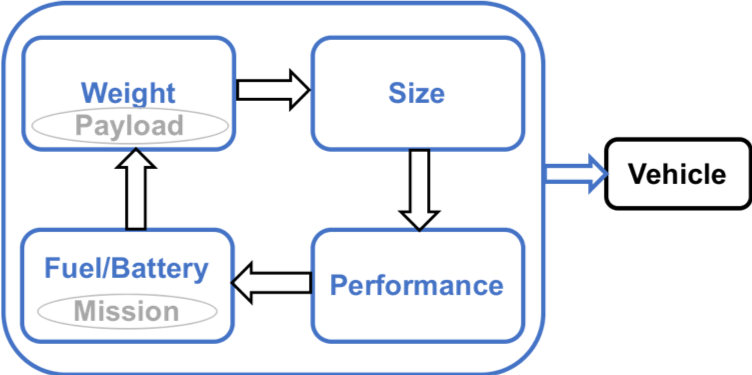
\includegraphics[width=0.65\textwidth]{images/iterate_loop.png}
\caption{Iterative sizing: the classical approach}
\label{fig:itsize1}
\end{center}
\end{figure}

\begin{figure}
\begin{center}
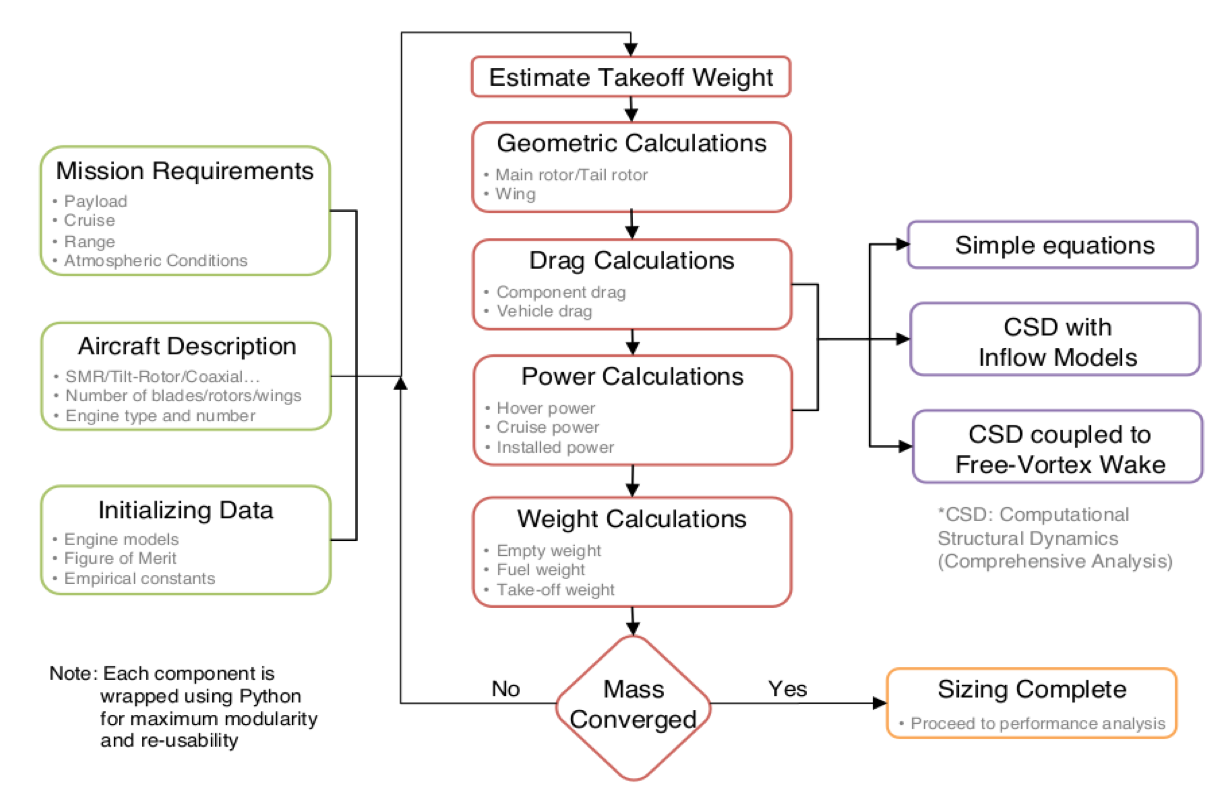
\includegraphics[width=\textwidth]{images/sizingloop.png}
\caption{Iterative sizing: detailed breakdown of operations}
\label{fig:itsize2}
\end{center}
\end{figure}

The \textbf{aircraft layout} is perhaps the most significant assumption required to initiate sizing. Figure~\ref{fig:evtols} shows a few candidate eVTOL configurations, with different permutations and combinations of rotor and wing technologies, as shown in Fig.~\ref{fig:evtol_types}. In \hydra, the constituent rotor and wing technologies are defined as primitive types. Based on user inputs, these technology combinations are superimposed in \hydra \spc to obtain the appropriate configuration. 

\begin{figure}
\begin{center}
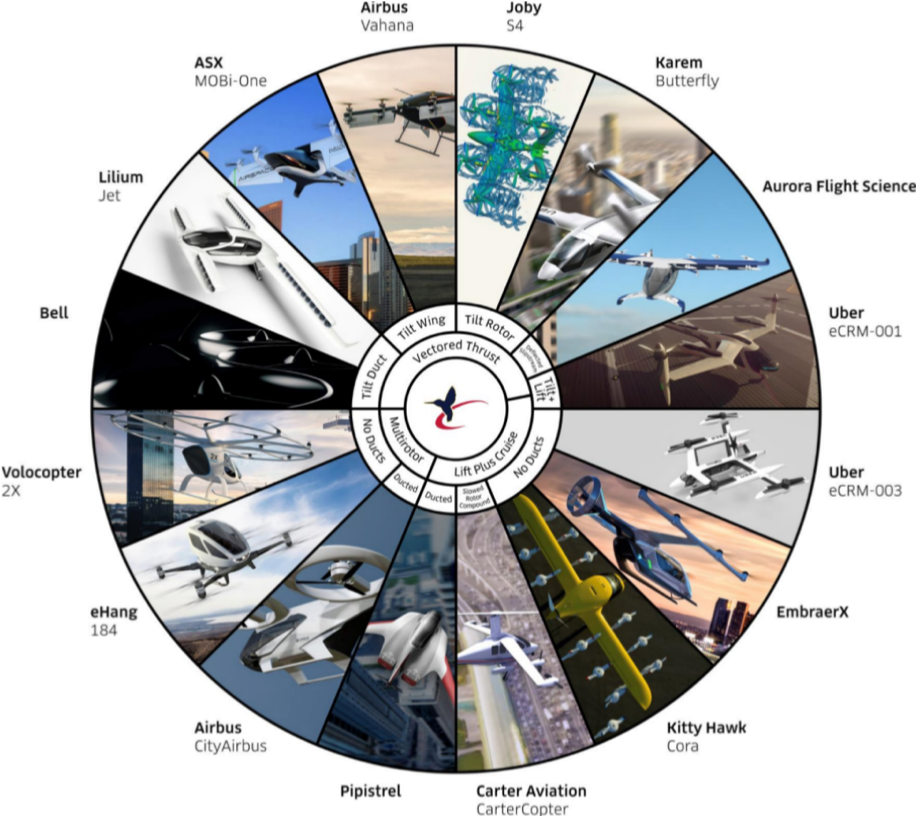
\includegraphics[width=0.75\textwidth]{images/evtols.png}
\caption{Variety in electric VTOL aircraft}
\label{fig:evtols}
\end{center}
\end{figure}

\begin{figure}
     \centering
     \begin{subfigure}
         \centering
         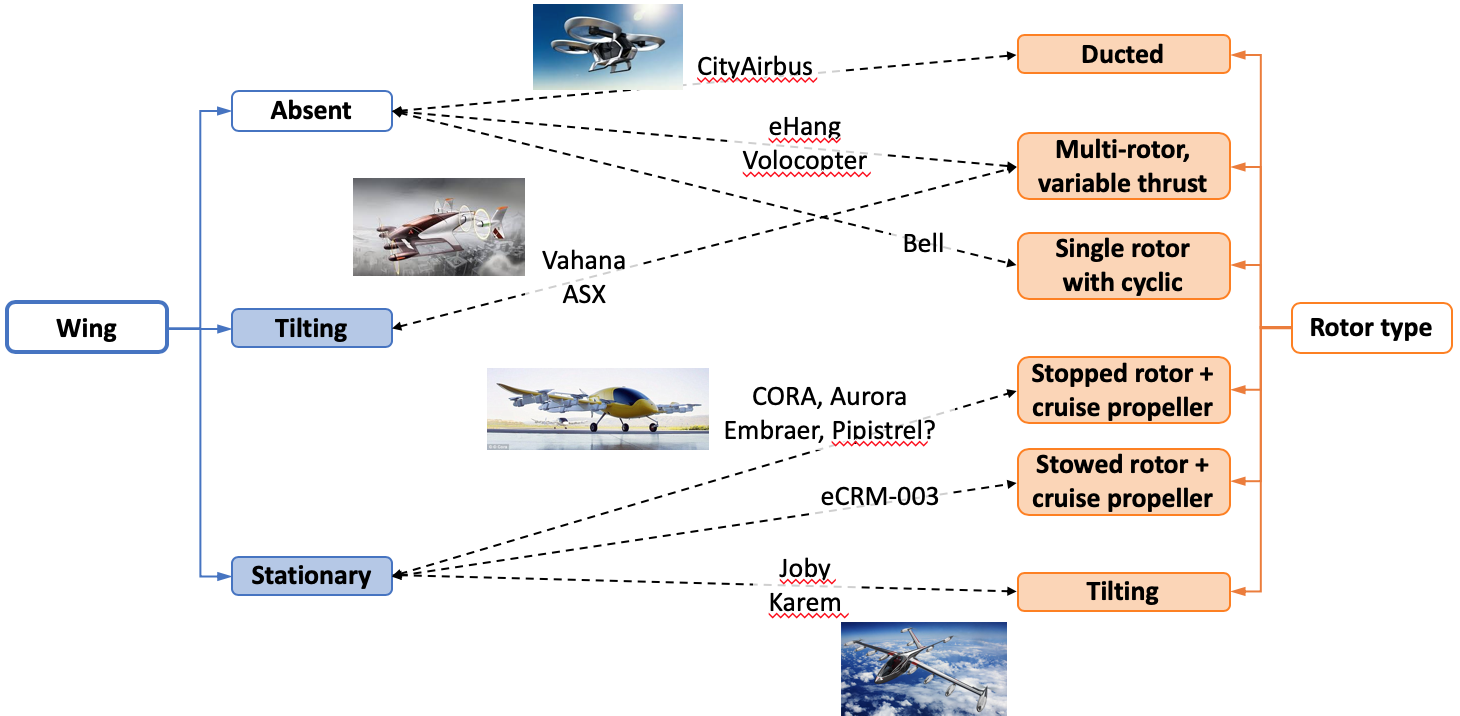
\includegraphics[width=\textwidth]{images/evtols1.png}
         \label{fig:evtols1}
     \end{subfigure}
     \hfill
     \begin{subfigure}
         \centering
         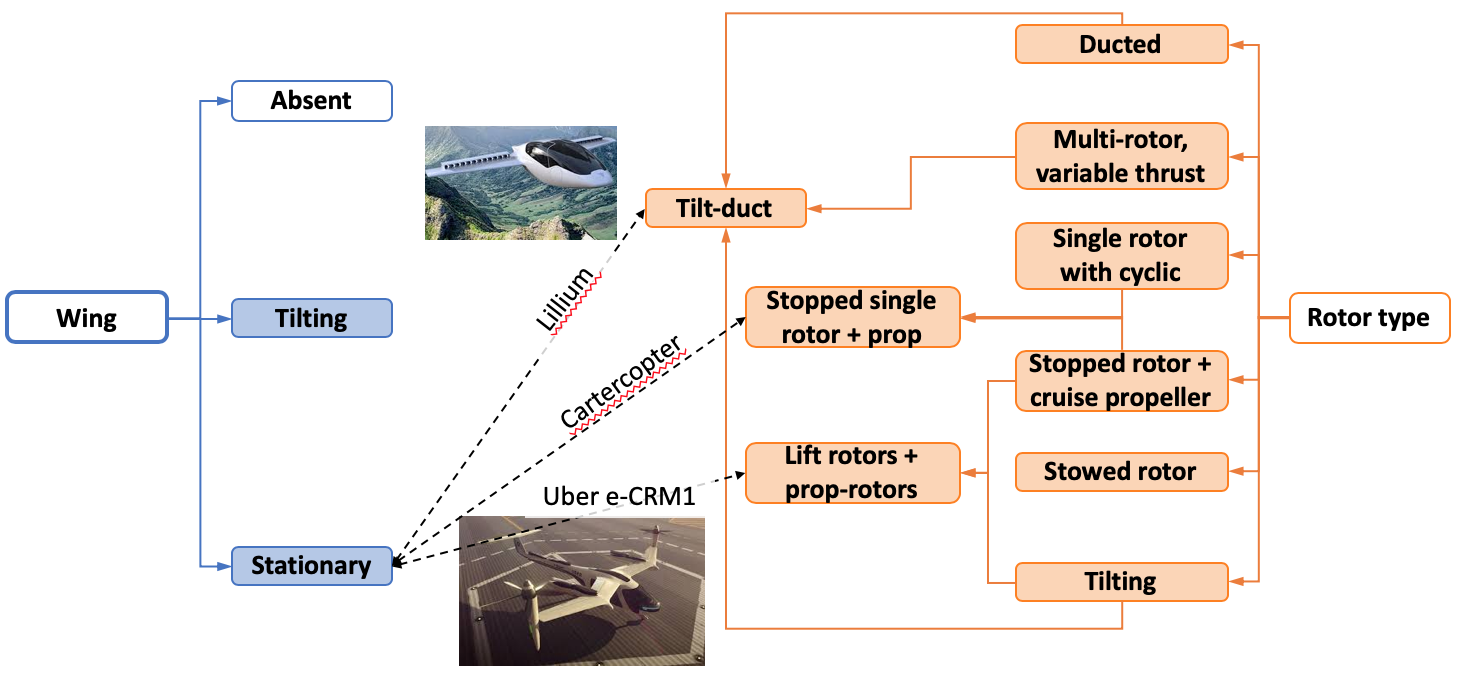
\includegraphics[width=\textwidth]{images/evtols2.png}
         \label{fig:evtols2}
     \end{subfigure}
        \caption{Assumbling eVTOLs from rotor and wing technologies}
        \label{fig:evtol_types}
\end{figure}

The \textbf{mission profile} is specified as a sequence of \textbf{hover} and \textbf{cruise} segments. Cruise segments are defined through a specified airspeed and distance/time, while hover segments are defined through duration. Climb and descent segments are defined as cruise segments with different start and end altitudes. An example mission profile is shown in Fig.~\ref{fig:mission}. 

\begin{figure}
\begin{center}
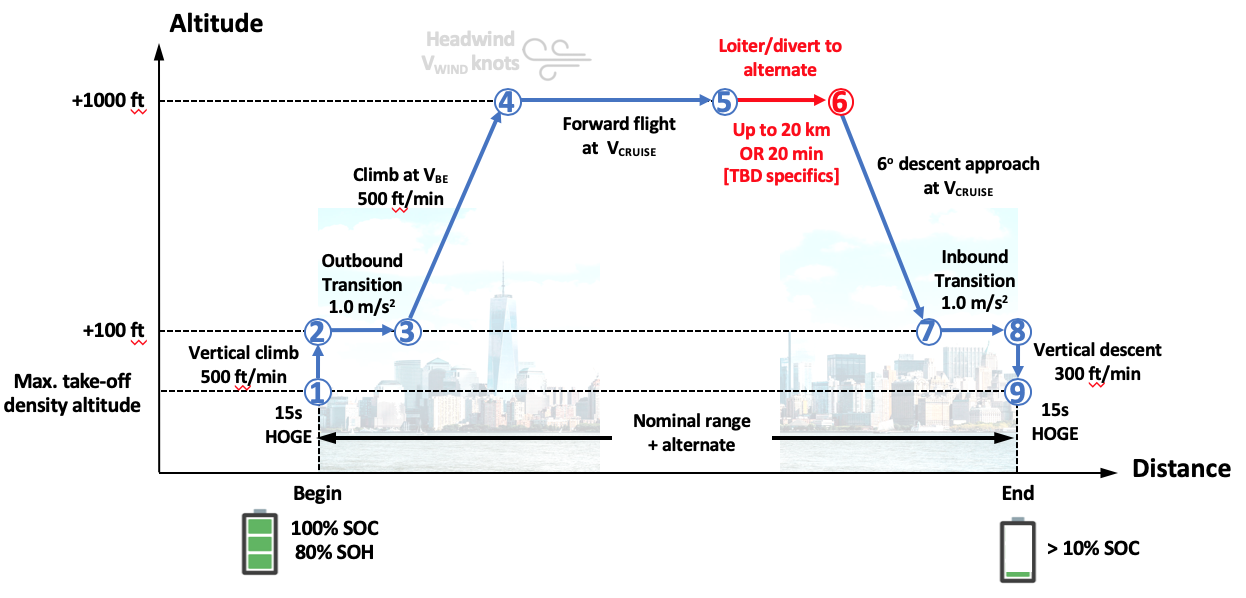
\includegraphics[width=\textwidth]{images/profile.png}
\caption{An example mission profile}
\label{fig:mission}
\end{center}
\end{figure}

Finally, the \textbf{model calibration data} refers to calibration constants for parametric models of rotor performance, turboshaft engine performance, electric motors, fuselage drag vs. weight curve fits, and several other assumptions. Typically, up to 30 constants are required to calibrate different low-fidelity models accurately, defined in the \textbf{defaults.yaml} input file. In \hydra, several parametric models have been systematically replaced with higher-fidelity counterparts and so lift the specific assumptions made to arrive at those constants. \\
\textbf{Accelerated convergence} \\
The implementation of iterative sizing shown in Fig.~\ref{fig:itsize1} requires several iterations (up to 30) to converge take-off mass to the required tolerance. An alternate approach is implemented in \hydra, resulting in significantly faster convergence for no loss in accuracy. This accelerated convergence technique is shown in Fig.~\ref{fig:accel_conv}. 

In this method, the ``inner loop'' is executed in fixed take-off mass mode, and the constituent weight groups are evaluated. Finally, the remaining mass (take-off mass minus empty weight, minus energy storage) is assigned to payload mass, i.e., 

\begin{equation}
\textrm{m}_{\rm pay} \quad = \quad \textrm{M} \spc - \spc \textrm{m}_{\rm empty} \spc - \spc \textrm{m}_{\rm battery} \spc - \spc \textrm{m}_{\rm fuel}
\end{equation}

\begin{figure}
\begin{center}
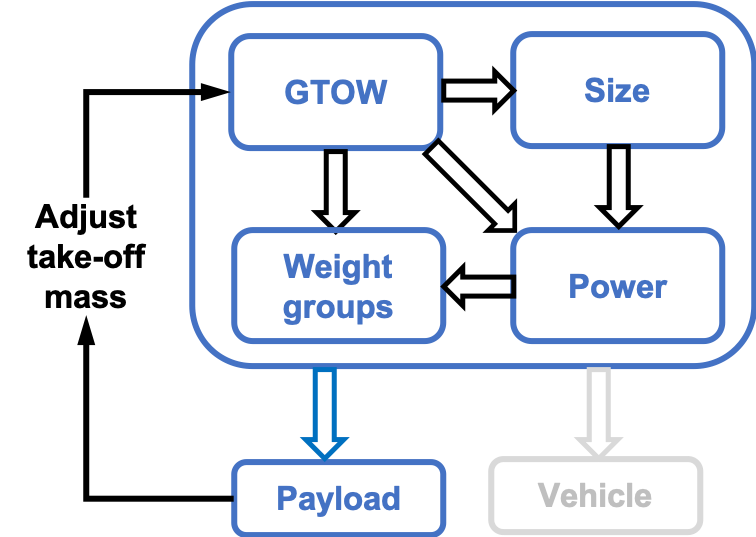
\includegraphics[width=0.5\textwidth]{images/accel_conv.png}
\caption{Accelerated convergence for iterative sizing}
\label{fig:accel_conv}
\end{center}
\end{figure}

Here, $M$ represents the take-off mass. Usually, mission profiles are specified together with the target payload m$_{\rm target}$. However, the ``inner loop'' described above runs once to calculate the payload mass m$_{\rm pay}$ for a given take-off mass $M$. Therefore, the take-off mass needs to be continuously adjusted to ensure that the ``calculated'' payload matches the target payload. One update scheme for the take-off mass (used in \hydra) is 
\begin{equation}
M_{i+1} \quad = \quad M_i - \frac{dM}{d\textrm{m}_{\rm pay}} (\textrm{m}_{\rm pay} - \textrm{m}_{\rm target})
\end{equation}
The slope $\frac{dM}{d\textrm{m}_{\rm pay}}$ is initially set to 3.0, and subsequently updated based on a finite-difference approximation as iterations proceed. This method usually converges in 3 -- 5 updates for take-off mass (vs. 30 iterations for the baseline technique), resulting in 5 -- 6 times faster convergence for no reduction in accuracy.

\subsubsection{Constrained optimziation}
The other technique that lends itself to VTOL conceptual sizing is constrained optimization. The primary advantage of this technique is that it allows for simultaneous minimization of a cost function (e.g. vehicle operating cost) while satisfying compatibility constraints (e.g., payload matching and landing footprint). If only sizing is required, the design variables are fed as prescribed inputs and compatibility constraints are specified as nonlinear algebraic constraints. The take-off weight is provided as a design variable and the payload is calculated as an output. The condition that the calculated payload (m$_{\rm pay}$) be at least the target mission payload (m$_{\rm target}$) is enforced as a nonlinear inequality constraint. 

In \hydra, two different optimizers are used for constrained minimization of the vehicle hourly operating cost: gradient-based optimization, and differential evolution. The constraints are landing footprint (based on wing span and fuselage length) and payload matching. For \textbf{concentual sizing}, gradient-based optimization requires an accurate initial condition to ensure that global minima (and not local minima) are identified at the end of optimization. In \hydra, the gradient-based optimizer is initialized from several starting conditions, each of which are obtained from a parametric sweep over the available high-level design variables. For \textbf{differential evolution}, compatibility constraints are implemented indirectly as a ``death penalty'' - an analog of exterior penalty functions. The cost function is increased by a large number (1e6) for designs that violate any of the user-specified constraints. Additionally, \hydra \spc is programmed to automatically add and remove design variables based on the number of rotor and wing groups in the vehicle. 

The optimizer in \hydra \spc is invoked after basic sizing over a limited parametric sweep is carried out. Both optimization techniques - gradient based and differential evolution - are used to minimize vehicle operating costs, and the resulting optimized designs are checked for uniqueness. These unique designs (obtained from optimization with different starting conditions) are ranked by operating cost, weight, battery/fuel or rated power based on a user-selected criterion. Further details are provided in the appropriate section later on in the documentation. 

\section{Drag models}

\subsection{Fuselage and empennage drag}
The fuselage is modeled as a slender body of revolution with its length set by user inputs, and an equivalent diameter based on body width and height (also set by the user). The procedure to calculate skin friction drag and base drag are identical to those documented in NASA CR-3083: \emph{ Rotary-Wing Aerodynamics: Volume II} by C.N. Keys. Similiarly, the approach for estimating the drag of horizontal and vertical tail surfaces, as documented in NASA CR-3083, is implemented in \hydra.

\subsection{Edgewise rotor hub drag}
The flat-plate area of each edgewise rotor hub is estimated based on a modified procedure outlined in NASA CR-3083, as follows:
\begin{equation}
f_{\rm hub} \quad = \quad 1.2 R^2 (0.0006 + 0.00222 N_{\rm b})
\end{equation}

\subsection{Spinner drag}

The spinner is assumed to be a rotating body with a hemispherical nose and blunt base. As shown in Fig.~\ref{fig:fus_drag}, the drag coefficient of such a shape is 0.2 (referenced to cross-sectional area $\pi d^2/4$), for a length-to-diameter ratio of 2.5. For the calculations presented in this paper, a drag coefficient of 0.36 is assumed, to account for additional blockage from the airframe, vertical fins and interference effects. The radius of the spinner is 15\% of the rotor radius. 

\begin{figure}
\begin{center}
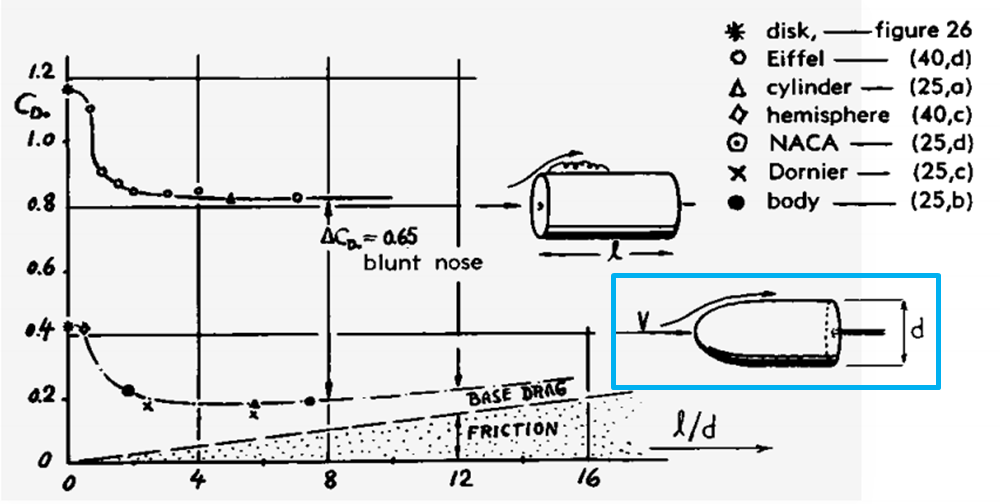
\includegraphics[width=\textwidth]{images/fus_drag.png}
\caption{Spinner nose cone:drag coefficient, from \emph{Fluid Dynamic Drag, Hoerner}}
\label{fig:fus_drag}
\end{center}
\end{figure}

\subsection{Momentum drag for engine air intakes}
For turboshaft engines operating at cruise speeds above 160 knots, the additional momentum drag is 0.3 ft$^2$ per intake.

\subsection{Landing gear drag}
The drag of landing gear is modeled with a parametric representation (obtained from NASA CR-3083) as follows:
\begin{equation}
\log_e f_{\rm LG} \quad = \quad y_0 + m \log_e(0.001 W)
\end{equation}

Here, $f_{\rm LG}$ is in square feet, and $W$ is in lbs. The constants $y_0$ and $m$ are set based on the type of landing gear. 
\begin{enumerate}
\item \textbf{Retracted gear}: $f_{\rm LG}$ = 0
\item \textbf{Wheeled gear}: $y_0$ = 0.5755. The slope $m$ = 0.443  for W $\geq$ 1000 lb, and zero for W $\leq$ 1000 lb.
\item \textbf{Skid gear}:  $y_0$ =-0.11626. The slope $m$ = 0.4979  for W $\geq$ 1000 lb, and zero for W $\leq$ 1000 lb.
\end{enumerate}

\subsection{Cooling drag}
The cooling systems required to regulate engine temperatures creates additional drag, which is estimated using a parametric model given in NASA CR-3083.
\begin{equation}
f_{\rm cool} ({\rm ft}^2)\quad = \quad 10^{-4} P_{\rm ins} (hp)
\end{equation}

\subsection{Mast fairing drag for coaxial rotors}
The fairing for the exposed length of the rotor shaft between the upper and lower rotors of a coaxial system incurs an additional drag penalty, given by 
\begin{equation}
f_{\rm mast} ({\rm ft}^2)\quad = \quad 0.0322 R^2
\end{equation}

\subsection{Protrusion drag}
The drag of protrusions is modeled as an additional 10\% of the accumulated parasitic drag of all wetted surfaces.

\section{Rotor and Wing Performance Models}

\subsection{Rotor performance model}

Two performance models are used to calculate rotor power required in hover and axial flight. The first model is based on momentum theory, and the second model is based on blade element momentum theory. 

\subsubsection{Momentum Theory}
For momentum theory-based predictions, rotor power is calculated based on assumed aerodynamic efficiency factors in hover and cruise. Imperial units (foot, pounds of force and horsepower) are assumed for these expressions. In hover, rotor power is given by 
\begin{equation}
P_{\rm hover} (hp) \quad = \quad \frac{T_R^{1.5}}{550 \sqrt{2 \rho A} \textrm{ FM}}
\end{equation}
Here, $T$ is the thrust required in hover from each rotor, and is calculated assuming the segment weight is equally divided between all rotors. A vertical download factor (configuration-dependent) is included in the estimation of rotor thrust. The rotor disk area is $A$ (ft$^2$), $\rho$ is the ambient air density (slug/ft$^3$) and FM is the rotor figure of merit in hover. 

In cruise, the power required by each rotor when operating in axial flight is 
\begin{equation}
P_{\rm cruise} (hp) \quad = \quad \frac{D}{N_{_\textrm{R}} } \frac{V_{\infty}}{550 \eta_{\rm p}}
\end{equation}

Here, $D$ is the total vehicle drag in lbs when operating at a forward flight speed of $V_{\infty}$ ft/s, which is overcome by each of the N$_{_\textrm{R}}$ rotors operating at a propeller efficiency of $\eta_{\rm p}$. 

%The assumed figure of merit $FM$ and propeller efficiency in cruise $\eta_{\rm p}$ are 0.7 and 0.8, respectively.

\subsubsection{Blade Element Momentum Theory (BEMT)}
Certain configurations like the tilt-rotor or tilt-wing fly such that the rotors operate predominantly in axial flight. Therefore, the Blade Element Momentum Theory (BEMT) is used as a higher-fidelity replacement for momentum theory-based predictions. Though BEMT can resolve finer details like angle of attack variations along the span, it requires detailed inputs, namely airfoil tables and distribution of blade chord and twist along the span. These details are populated as described below.

The rotor is assumed to be constructed from multiple user-specified airfoils. The lift and drag characteristics for each airfoil may be Reynolds-tabulated or mach-tabulated. Several combinations of blade chord and twist distribution are generated assuming linear taper and bilinear twist. The design variables for blade geometry are:
\begin{enumerate}
\item Blade taper ratio (1:1, 2:1 and 3:1)
\item Blade bilinear twist junction (30\% -- 70\% span)
\item Twist at bilinear junction (-5 deg to -20 deg)
\item Twist at tip (-5 deg to -35 deg)
\end{enumerate}
The rotor RPM in cruise (specified as a fraction of hover RPM) is added as a sizing variable. The BEMT analysis calculates the rotor power required for a given thrust, for all mission segments, exploring a parameter space of 360 designs (combinations of blade twist and taper distribution). The rotor geometry for minimum energy consumption over the mission is identified from the parametric sweep, and the aerodynamic efficiencies (figure of merit $FM$ in hover and propeller efficiency $\eta_{\rm p}$ in cruise) are calculated for each mission segment. 

Minimizing the energy required at the rotor ensures reduced fuel consumption, but not necessarily a good overall design. A cruise-dominated mission results in a prop-rotor with a potentially degraded hover figure of merit while achieving good aerodynamic cruise efficiency. Therefore, installed power (and therefore, engine and transmission weights) may increase, resulting in a lower payload fraction. To prevent unchecked increases in powerplant weights, another condition is introduced in the BEMT analysis: designs are considered ``valid" if the hover figure of merit is greater than a user-specified threshold (e.g., 0.72), and only these valid designs are ranked to determine the ``best'' rotor efficiencies.

When BEMT is included in the sizing iterations, sizing proceeds in 3 steps:
\begin{enumerate}
\item Perform sizing with momentum theory and assumed efficiency factors in hover and cruise ($FM$=0.75, $\eta_{\rm p}$=0.82)
\item If the design satisfies all constraints, perform BEMT analysis to calculate aerodynamic efficiencies for each segment based on thrust requirements; extract hover or cruise efficiencies (FM, $\eta_{\rm p}$).
\item Perform sizing with momentum theory, using the calculated rotor aerodynamic efficiencies obtained in Step 2.
\end{enumerate}

%When BEMT is included in sizing, the rotor performance calculations are the bottlenecks for computational efficiency; 8 designs can be sized in one second, compared to 50 designs per second when using momentum theory with the FEA-based airframe weight model.

\begin{figure}
\centering    
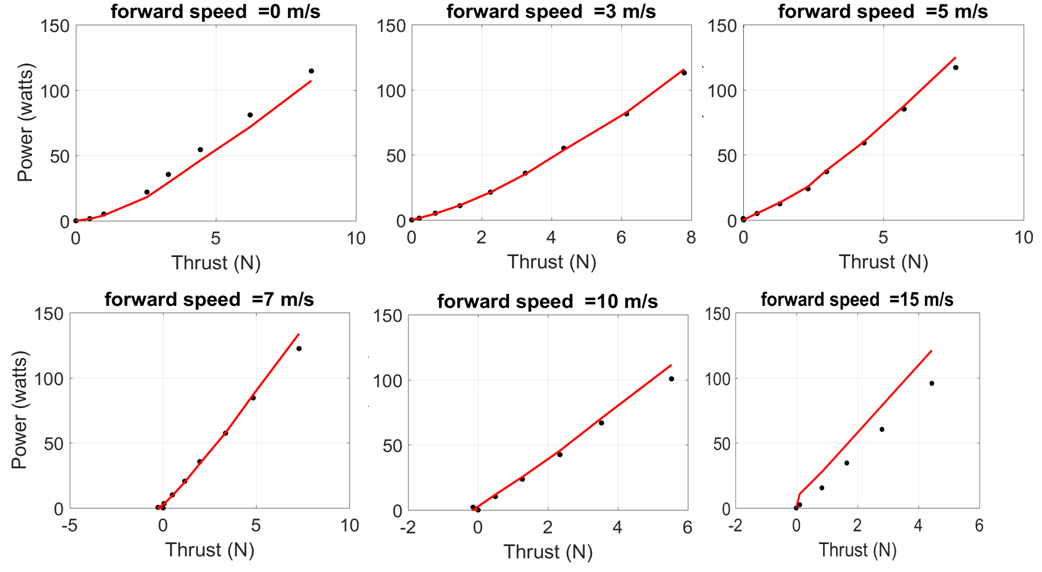
\includegraphics[width=\textwidth]{images/bemt_validation.png}
\vspace{-1cm}
\caption{Comparison of BEMT predictions to experiments}
\label{fig:bemt}
\end{figure}

Figure~\ref{fig:bemt} shows the comparison of thrust and power obtained from BEMT predictions with airfoil tables vs. sub-scale experiments for a variable-pitch and variable-RPM sub-scale prop-rotor. Good predictions were obtained at various cruise speeds ranging from 3 m/s to 15 m/s. For these cases, BEMT was found to be sufficient for accurate performance predictions. %The rotor geometry and details of the experiment were obtained from Ref.~\citenum{Phillips16}.

\subsection{Wing performance model}
The drag coefficient of a fixed wing is given by 
\begin{equation}
C_D \quad = \quad C_{Do} \spc + \spc \frac{1}{\pi AR e} C_L^2 
\end{equation}
The lift coefficient $C_L$ and aspect ratio $AR$ are sizing design variables. The profile drag coefficient $C_{Do}$ is an assumed value, usually 0.014 (including protrusions and interference). The Oswald efficiency $e$ is calculated as %using the methodology of Kroo, summarized by Nita and Scholz as follows:
\begin{align*}
e \quad &= \quad \left(Q + P \pi AR \right)^{-1}  \\
P \quad &= \quad 0.38 \times 0.02 \\
Q \quad &= \quad \frac{1.01}{s} \\ 
s \quad &= \quad 1 \spc - \spc 2 \left(\frac{d_{\rm fus}}{b_{\rm wing}}\right)^2
\end{align*}
The parameters are $d_{\rm fus}$ = equivalent fuselage diameter, and $b_{\rm wing}$ = wing span.
\pagebreak
\section{Weight models}
There are three main contributors to vehicle take-off mass:
\begin{enumerate}
\item {\bf Energy storage} - battery and/or fuel weight. This component may be traded-off against payload for mission flexibility, depending on available volume. 
\item {\bf Empty weight} - this weight group represents the airframe, wings, rotors, engines, transmission, motors, seats, avionics and other non-removable systems.
\item {\bf Payload} - usually specified with the mission definition.
\end{enumerate}

\subsection{Engines, fuel and batteries}
Though engines strictly belong in the empty weight category, the calculation of fuel weights are inextricably linked to the evaluation of engine performance and engine weights. Therefore, engine models are described in this section. 

\subsubsection{Engines}
\hydra \spc has built-in models for fuel-burning engines of two types: gas turbine engines, and reciprocating engines (piston engines and aero-diesel engines). \\
\textbf{Turboshaft engines} \\
Based on statistical data for various production engines, a trend line was fitted with good accuracy ($R^2 = 0.92$) for the variation of engine weight W$_{\rm engine}$ (lb) with installed power P$_{\rm ins}$ (hp). The fitted engine weight model is given by
\begin{equation}
\label{eqn:turbowt}
W_{\rm engine}\spc (\textrm{lb}) \quad = \quad 7.3874 \textrm{ P}_{\rm ins}^{0.552}
\end{equation}
Another fit is shown in Fig.~\ref{fig:turboshaft}, in SI units with engines manufactured over the last fifty years.

The variation of engine Specific Fuel Consumption (SFC) at peak efficiency with installed power is 
\begin{equation}
\textrm{sfc}_{_{\rm base}} \spc (\textrm{lb/hp-hr}) \quad = \quad 1.549 \textrm{ P}_{\rm ins}^{-0.161}
\end{equation}
Engines operating at sub-optimal conditions (i.e. at power settings lower than design power output) suffer from higher specific fuel consumption. This effect is modeled using a power law as 
\begin{equation}
\label{eqn:sfcpower}
\textrm{sfc} \quad = \quad \textrm{sfc}_{_{\rm base}} \left(\frac{\textrm{P}_{\rm req}}{\textrm{P}_{\rm ins}}\right)^{-0.256}
\end{equation}
Here, P$_{\rm req}$ is the power output required from the engine to produce a thrust $T$ during a mission segment. Finally, the variation of available power (relative to installed power) with ambient temperature and pressure is given by 
\begin{equation}
\textrm{P}_{\rm avail} \quad = \quad \textrm{P}_{\rm ins} \spc [1 - K_T (\theta-1)] \spc [1 + K_D (\delta-1)]
\end{equation}
The terms $\theta$ and $\delta$ are ratios of ambient temperature and ambient pressure to their corresponding values at mean sea level (ISA). The constants $K_T$ and $K_D$ are obtained from curve fits of detailed engine performance curves. \\
\begin{figure}
\begin{center}
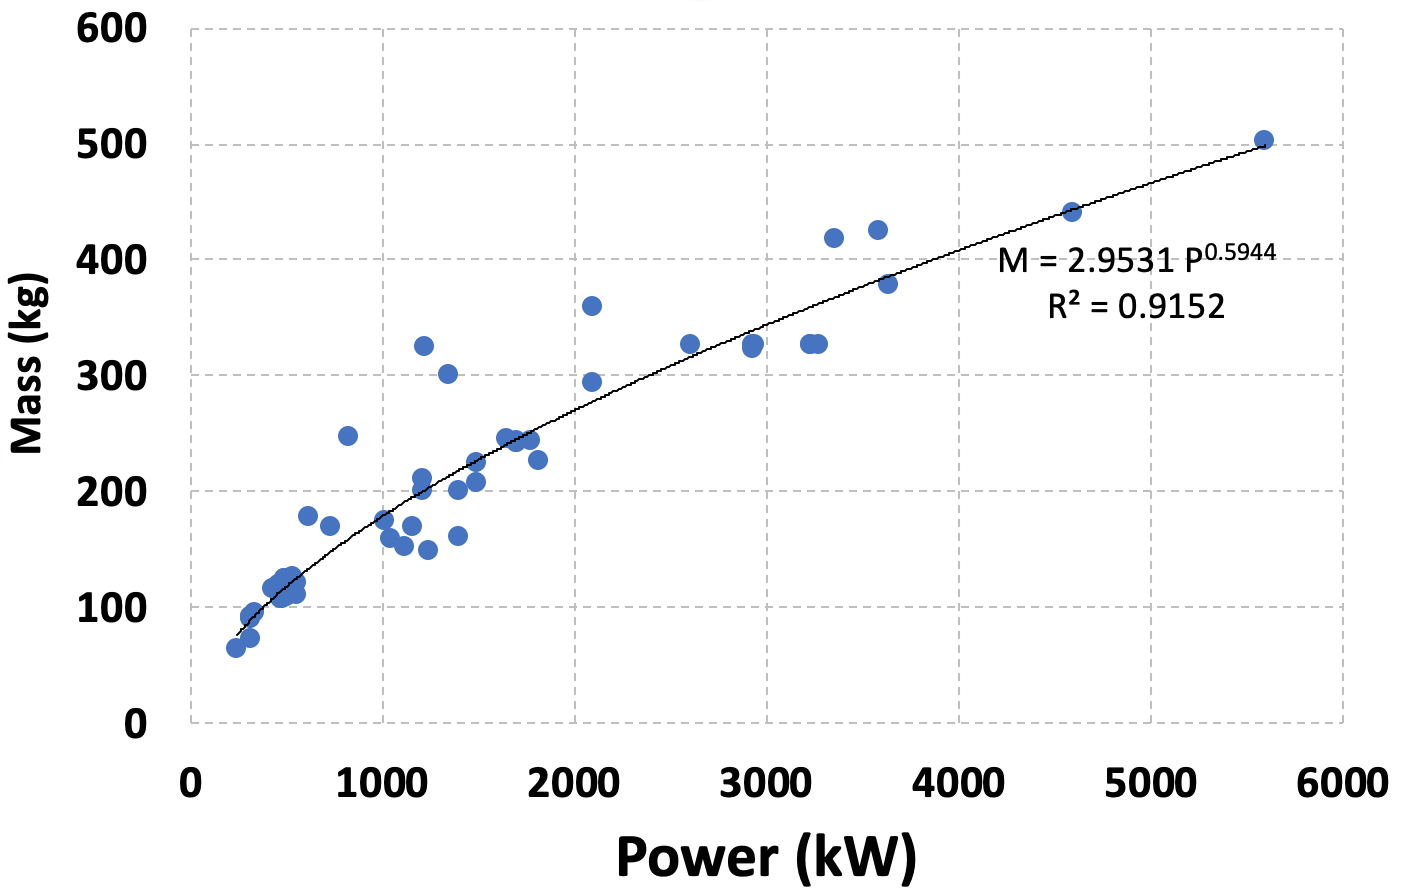
\includegraphics[width=0.75\textwidth]{images/turboshaft.png}
\vspace{-0.1cm}
\caption{Statistics: turboshaft engine mass vs. installed power}
\label{fig:turboshaft}
\end{center}
\end{figure}
\textbf{Piston engines} \\
The treatment of piston engine weights is similar to that followed for turboshaft engines. The variation of engine weight with installed power is given by 

\begin{equation}
\label{eqn:pistonwt}
W_{\rm engine}\spc (\textrm{lb}) \spc = \spc 2.367 \textrm{ P}_{\rm ins}\textrm{ (hp)} ^ {0.916} \quad 35 \leq \textrm{ P}_{\rm ins}\textrm{ (hp)} \leq 1000
\end{equation}
Another fit is shown in Fig.~\ref{fig:piston}, in SI units with a larger sample size, including less efficient engines. The variation of engine SFC at its peak efficiency is 
\begin{align*}
\textrm{sfc}_{_{\rm base}} (\textrm{lb/hp-hr}) \spc = &\spc 0.42, \spc \textrm{ P}_{\rm ins} \textrm{ (hp)} \leq 4 \\
=&\spc 0.594 - 0.0046 \textrm{ P}_{\rm ins} \textrm{ (hp)}, \spc 4 \leq \textrm{ P}_{\rm ins} \leq 56 \\
=&\spc 0.52 \textrm{ P}_{\rm ins} \textrm{ (hp)}^{-0.0972}, \spc 56 \leq \textrm{ P}_{\rm ins} \leq 1000
\end{align*}

\begin{figure}
\begin{center}
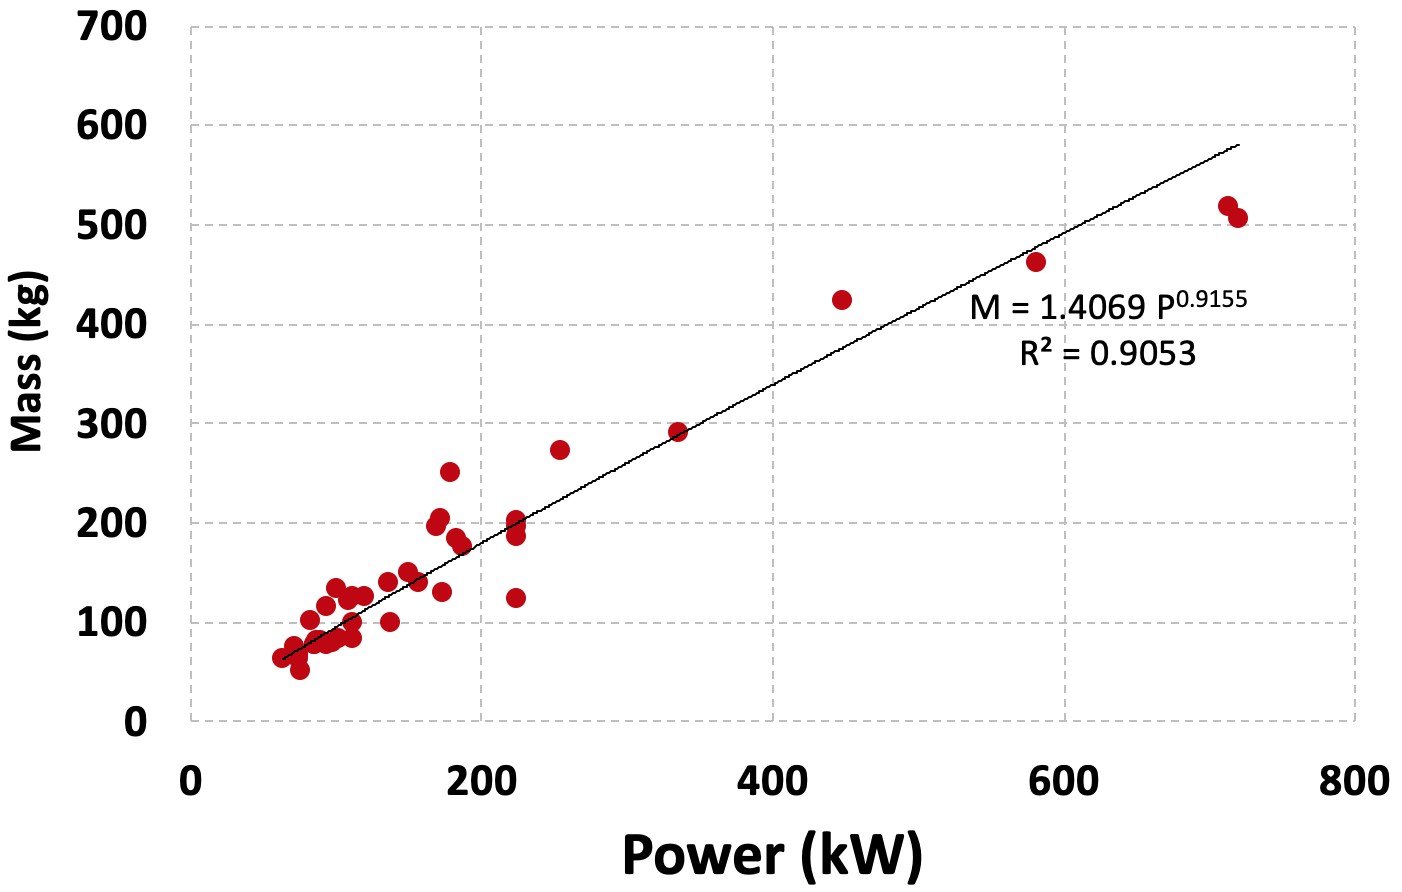
\includegraphics[width=0.75\textwidth]{images/piston.png}
\vspace{-0.1cm}
\caption{Statistics: reciprocating engine mass vs. installed power}
\label{fig:piston}
\end{center}
\end{figure}

%Increases in engine SFC based on the operating condition are modeled similar to efficiency degradation of the turboshaft engine as given in Eqn.~\ref{eqn:sfcpower}.
\subsubsection{Fuel, tank and fuel handling systems}
After calculating the engine power required, the mission profile (flight segment duration) is used with engine power requirement and SFC estimates to calculate the fuel weight as 
\begin{equation}
m_{\rm fuel} \quad = \quad \mathlarger{\mathlarger{\Sigma}}_{i=1}^{\rm N_{\rm SEG}} \spc sfc(i) \spc P_{\rm eng}(i) \spc + \spc m_{\rm unusable}
\end{equation}
An average density of 6.7 lb/gal is used for both turbine engine fuel and aviation gasoline. The fuel tank and plumbing mass is estimated from fuel volume using AFDD models as 
\begin{equation}
   W_{\rm tank} \quad = \quad 0.4341 \spc V_{\rm tank}^{0.7717} \spc N_{\rm tank}^{0.5897}  \spc f_{\rm cw} \spc  f_{\rm bt}^{1.9491}
\end{equation}
The terms used in the equations are \\
V$_{\rm tank}$ is the tank volume in U.S. gallons (1 gal = 3.7.8 liters)\\
N$_{\rm tank}$ is the number of internal tanks \\
$f_{\rm cw}$ is the crashworthiness mark-up factor, usually 1.31 \\
$f_{\rm bt}$ is the ballistic survivability mark-up factor (1.2 for military, 1.0 for civilian) 

The weight of plumbing systems used for regulating fuel flow from tanks to engines is modeled as follows:
\begin{align*}
k0_{\rm plumb} \quad &= \quad \textrm{max}(0.022 M, 120) \\
k1_{\rm plumb} \quad &= \quad 0.025 k0 \\
W_{\rm plumb} \quad &= \quad k0_{\rm plumb} + k1_{\rm plumb} (0.01*N_{\rm tank} + 0.06*N_{\rm engine}) \spc \dot{V}^{0.866}
\end{align*}
$\dot{V}$ is the peak fuel flow rate to the powerplant in lb/hr and the plumbing system weight is in pounds. $M$ is the take-off mass in kg - the mixing of units and conventions is a result of AFDD models being specified in FPS units, while \hydra \spc is implemented in SI units. 

For small-scale powerplants, the trendlines predict an over-estimate of fuel handling system weight. To handle these special cases, a maximum limiter is placed on the fuel system weights, with the limit set to 50\% of fuel weight. 

\subsubsection{Battery models}
Battery weights are accurately represented using a very simple statistical model. Figure~\ref{fig:smallbattery} shows the variation of battery weight with rated energy capacity for commercially available small-scale batteries, where each data point represents a manufactured unit. Arguably, a battery density of 158 W-hr/kg is quite low and improvements can be made;  this ``conservative'' design is typical of commercially available battery packs including the safety casing. 

\begin{figure}
\begin{center}
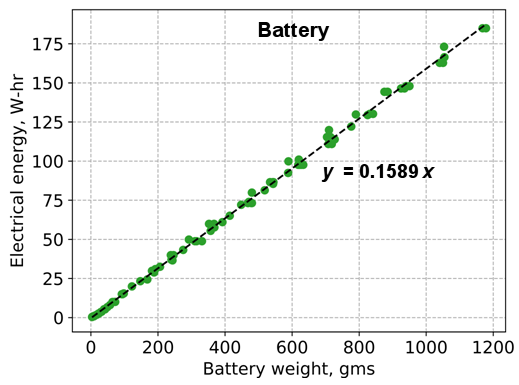
\includegraphics[width=0.75\textwidth]{images/battery.png}
\vspace{-0.1cm}
\caption{Small-scale batteries: weight statistics}
\label{fig:smallbattery}
\end{center}
\end{figure}

For full-scale platforms used in commercial operations, several conservative assumptions are used to incorporate various margins in sizing the battery. 
\begin{enumerate}
\item The minimum depth of discharge is 7.5\% of total energy capacity
\item The maximum state of charge near end of life for the battery is 80\%, i.e., after cycling, the usable battery capacity is at most 80\% of the rated energy. Thus, the effective usable energy for battery sizing is \textbf{72.5\% of the rated capacity}. 
\item The average discharge efficiency of the battery reduces by 4\% for every unit increase in average C-rating. 
\item A specific energy of 240 Wh/kg is used to estimate the mass of the cells.
\item A pack integration factor of 0.75 (defined as battery mass to cell mass) is used to estimate the weight of battery management systems and casing.
\item A curve fit of temperature rise vs. C-rating (obtained from experimental data) is used to track the rise of cell temperature over the mission duration. A maximum  limit of of 70$^o$C is used to iteratively add cells until thermal limits are satisfied.
\end{enumerate}

\subsubsection{Electric motor weights}
Though electric motor weights are strictly driven by peak torque requirements, the data correlation between weight and peak rated power is also very good as shown in Fig.~\ref{fig:smallmotor}. For small-scale motors, the speed controller is sized based on the current drawn by the system assuming a 12 Volt source. The masses of several large-scale motors with controllers are plotted against rated power in Fig.~\ref{fig:dcmotor}. Motor + speed controller efficiencies range from 85\% to 92\% depending on the design point and operating RPM range. Motor and speed controller weights are estimated as 
\begin{align*}
W_{\rm motor} (lb) \spc = & \spc 0.74 \textrm{ P} \qquad \qquad \qquad \textrm{P} \leq 13.4 \textrm{ hp} \\
W_{_\textrm{ESC}} (lb) \spc = & \spc 1.047 \textrm{ P} \qquad \quad \qquad \textrm{      P} \leq 13.4 \textrm{ hp}\\
W_{\rm motor} + W_{_\textrm{ESC}} (lb) \spc = & \spc 1.489  \textrm{ P}^{0.783} \quad 13.4 \textrm{ hp} < \textrm{P} \leq 350 \textrm{ hp}
\end{align*}

\begin{figure}
\begin{center}
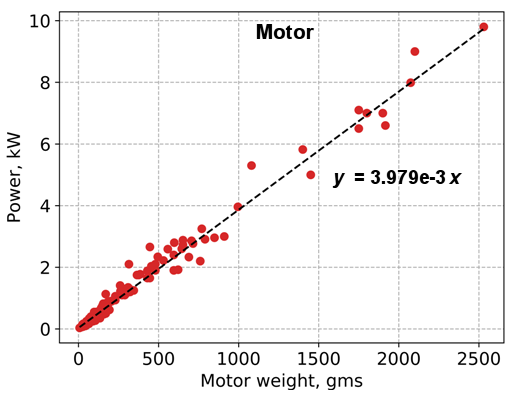
\includegraphics[width=0.75\textwidth]{images/motor.png}
\vspace{-0.1cm}
\caption{Statistics: weight of small BLDC motors}
\label{fig:smallmotor}
\end{center}
\end{figure}

\begin{figure}
\begin{center}
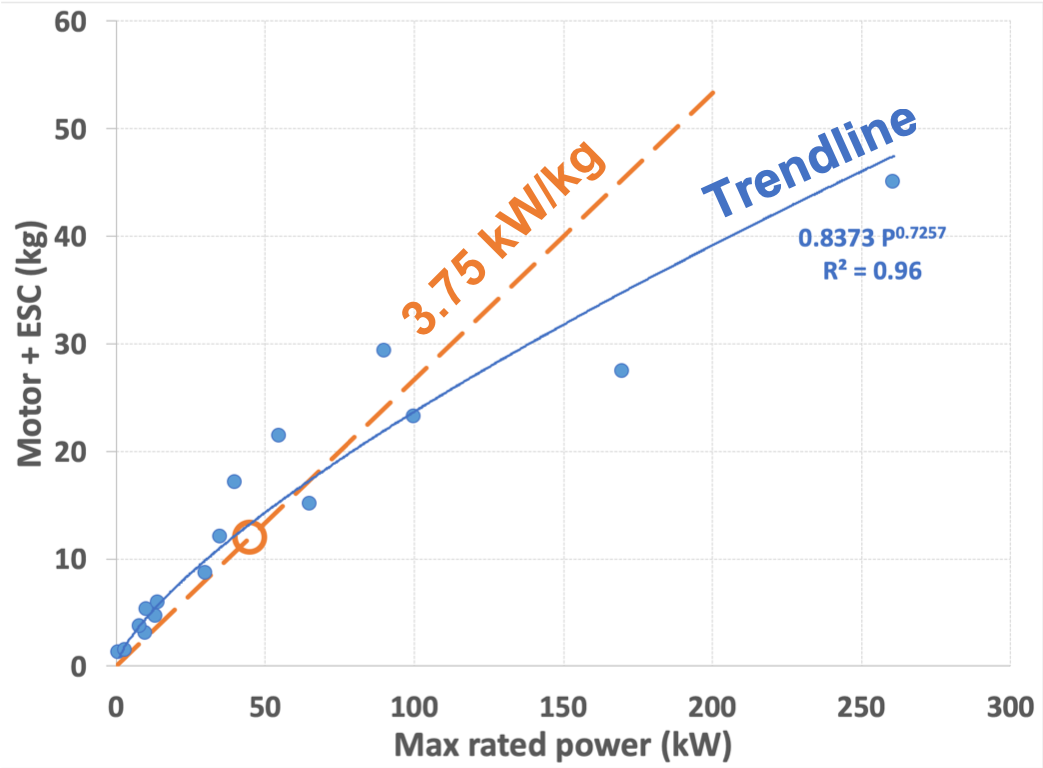
\includegraphics[width=0.75\textwidth]{images/dcmotor.png}
\vspace{-0.1cm}
\caption{Statistics: large-scale DC motor + controller mass vs. installed power. Manufacturing technology in 2018 can achieve 3.75 kW/kg of power density.}
\label{fig:dcmotor}
\end{center}
\end{figure}


 %For prop-rotors, the hover point is usually chosen as the operating condition for maximum efficiency (92\%), with the cruise point being chosen for lower motor efficiencies. 

\subsection{Electric Transmissions}
Generators for electric transmissions are sized in a manner identical to electric drive motors. The components of an electric transmission are shown in Fig.~\ref{fig:eltrans}.

\begin{figure}
\begin{center}
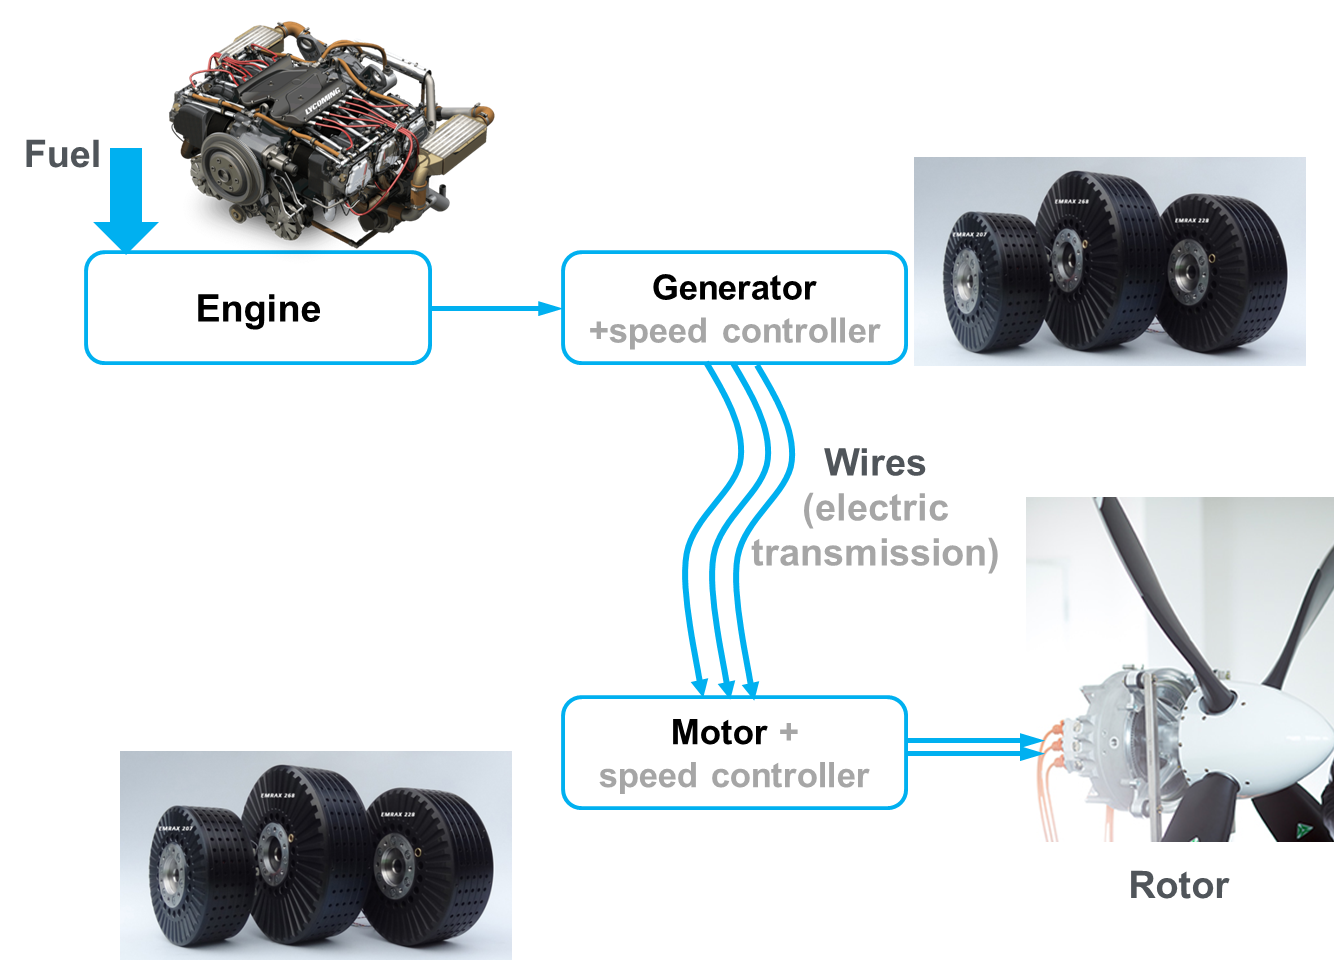
\includegraphics[width=0.75\textwidth]{images/eltrans.png}
\vspace{-0.1cm}
\caption{Turbine-generator hybrid powerplant for electric motor. 98\% wire transmission efficiency, 92\% generator efficiency}
\label{fig:eltrans}
\end{center}
\end{figure}

The advantage of this hybrid system is that a mechanical transmission is not required for power transmission to the rotors; further the hybrid system can serve as a long-range drop-in upgrade for short-range battery-powered variants. The disadvantage of a turboshaft-electric hybrid system is that each additional component introduces additional points of failure. Adding redundancy and fail-safe architectures can incur a significant empty weight penalty.

\subsection{Wire weights}
Two types of wires are considered in the sizing analysis: power cables and signal wires. The weights of electrical power cables are estimated from the vehicle rotor layout using a wire mass per unit length per unit power of 0.0057 kg/kW/m. Signal wires are calculated using a linear mass density of 0.17 kg/m and a knowledge of the rotor layout, together with an estimate of channel counts. Based on user inputs, doubly/triply redundant power cables and signal wires are automatically added to the appropriate weight groups for estimating vehicle empty mass.

At full-scale, a key driver of vehicle weight is the rotor design parameter set (tip speed, solidity, disk loading/radius, first rotating flap frequency). One such empirical parameter is the flap natural frequency. In the legacy approach for estimating rotor blade weight, the designer had to prescribe this parameter to perform sizing. However, underlying data for the flap frequency is restricted to articulated and hingeless rotors, and plentiful data is not available for stiffer rotors ($\nu_\beta \geq$ 1.08/rev). For small-scale VTOL with very stiff rotor systems ($\nu_\beta$ $\geq$ 1.4/rev), extrapolation of the trend line beyond the range of available data for $\nu_\beta$ may yield erroneous estimates for rotor blade weight. For eVTOLs, a physics-based approach is implemented and used in \hydra.

\subsection{Physics based model for rotor blades}

\begin{figure}
\begin{center}
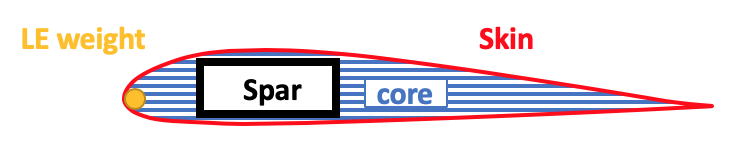
\includegraphics[width=0.75\textwidth]{images/cross_section.png}
\vspace{-0.1cm}
\caption{Blade cross-section}
\label{fig:cross_section}
\end{center}
\end{figure}

A schematic of the rotor airfoil is shown in Fig.~\ref{fig:cross_section}. The cross-section consists of two categories of materials: non-structural masses, and load-bearing components. The non-structural masses are:
\begin{enumerate}
\item Paint: 0.15 mm thickness, density 1800 kg/cu.m, applied on surface
\item Glue: 0.25 mm thickness, density 1800 kg/cu.m, applied on skin, shear webs
\item Core: density of 52 kg/cu.m, encompasses cross-section area of 0.49 $\left(\frac{t}{c}\right) c$
\item Leading edge protection: 1.14mm thickness, density 8900 kg/cu.m, from leading edge to 25\% chord on upper and lower surfaces.
\end{enumerate}
Here, $\left(\frac{t}{c}\right)$ is the airfoil thickness-to-chord ratio, usually 0.1 to 0.12 and $c$ is the blade airfoil chord. For the paint and glue, the chordwise location of the component center of gravity is 0.5$c$. For the leading edge protection strip and core, the component chordwise center of gravity locations are 12.5\% chord and 57\% chord, respectively. 

\subsubsection{Skin sizing}
The skin is sized to withstand a total torsion moment equivalent to an airfoil $c_m$=0.2 at the maximum rated rotor speed. The total root pitching moment in hover is 
\begin{equation*}
M_x \quad = \quad \frac{1}{6} \rho V_{\rm TIP}^2 c^2 c_m R 
\end{equation*}
The skin thickness is given by 
\begin{equation*}
t_{\rm skin} \quad = \quad \frac{n M_x}{2 A_{\rm cs} \tau_{\rm skin}}
\end{equation*}
Here, $A_{\rm cs}$ is the cross-section area of the airfoil, and $\tau_{\rm skin}$ is the maximum allowable shear stress in the skin. The factor $n$ accounts for additional overload and safety factors to account for for contingency conditions and fatigue margins. 

\subsubsection{Leading edge weight}
The section chordwise center of gravity for the non-structural components (paint, leading edge protection and core) along with the skin is obtained from the respective weights and component centroid locations. If this center of gravity is behind the blade quarter-chord, a leading edge weight is added to avoid torsional divergence  and flutter for the blade.

The CG of the non-structural components and skin is given by 
\begin{equation*}
\frac{x_1}{c} \quad = \quad \frac{\quad m_{\rm LEP} 0.125 \pls  m_{\rm skin} 0.5 \pls m_{\rm core}  0.57 \pls m_{\rm paint} 0.5 \pls m_{\rm glue} 0.5}{m_{\rm LEP} \pls m_{\rm skin} \pls m_{\rm core} \pls m_{\rm paint} \pls m_{\rm glue}}
\end{equation*}

If $\frac{x_1}{c}$ is greater than 0.25, then a leading edge mass is added, equal to 
\begin{equation*}
m_{\rm LE} \quad = \quad (m_{\rm LEP} \pls m_{\rm skin} \pls m_{\rm core} \pls m_{\rm paint} \pls m_{\rm glue}) \spc \left(4 \frac{x_1}{c} \spc - \spc 1\right)
\end{equation*}

\subsubsection{Spar caps and shear web sizing}
The spar is placed so that the neutral axis and CG both lie at quarter-chord. A NACA-0012 section is used to estimate The elements that support shear and bending moment due to lift and drag and bending loads are the spar webs (shear and lag bending moment) and spar caps (flap bending moment and tension due to the centrifugal load). 

The limit load for eVTOL rotor blades is determined from the trim thrust required under OMI (One Motor Inoperative) conditions. For the ``conventional'' tilt-wing configuration (6 rotors on main wing, 2 rotors on horizontal tail) and the tandem tilt-wing configuration (4 rotors each on canard and wing), the maximum thrust scaling factor is approximately 150\% the hover thrust. With rotor radius $R$, rotor speed $\Omega$ and peak torque at the blade root $Q_b$ determined from the rotor geometry, the vertical force on the blade is obtained by dividing the maximum expected thrust level by the total number of blades as 
\begin{equation}
F_z \quad = \frac{W}{N_R N_b} n_z
\end{equation} 
The terms $n_z$ is a load factor that can incorporate safety margins, dynamic overshoot/landing and fatigue factors for blade loads. The lift distribution along the span is assumed to be quadratic (a structurally conservative loading profile - the optimum hovering rotor features a linear spanwise lift distribution, discounting tip loss effects). The blade is assumed to constructed with a pre-cone angle $\beta_p$ to alleviate root bending moments, and then subdivided into $N=5$ equal span segments. One such segment is shown in Fig.~\ref{fig:blade_segment}.

\begin{figure}
\begin{center}
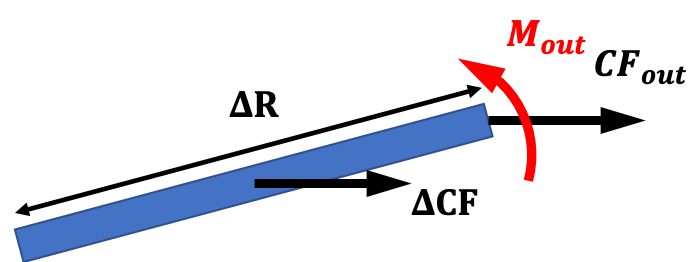
\includegraphics[width=0.75\textwidth]{images/blade_segment.png}
\vspace{-0.1cm}
\caption{Blade spanwise segment}
\label{fig:blade_segment}
\end{center}
\end{figure}

The dominant loads on the outboard end of the segment, that are carried by the spar caps, are the centrifugal force (from all segments outboard of the present one) and a flap bending moment due to (i) distributed lift on segments outboard of the present one, and (ii) a combination of pre-cone and centrifugal load on segments outboard of the present one. The blade spanwise segments are successively sized starting from the tip segment and ending in the root segment. A schematic of the rotor blade segment and cross-section is shown in Fig.~\ref{fig:blade_sizing}.

\begin{figure}
         \centering
		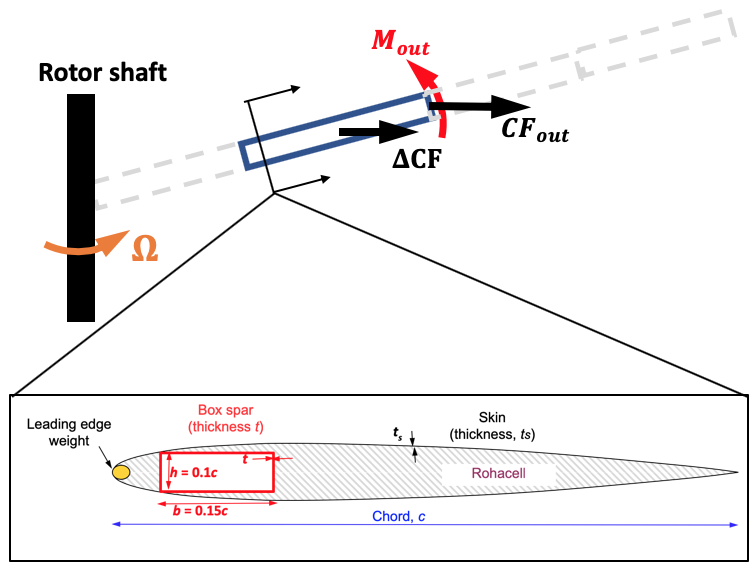
\includegraphics[width=0.7\textwidth]{images/rotor_sizing.png}
        \caption{Rotor blade segment sizing: schematic}
        \label{fig:blade_sizing}
\end{figure}

The total centrifugal load and flap bending moment at the inboard end of the segment is 
\begin{align}
\label{eqns:cfbma}
CF(x_{\rm in}) \quad &= \quad CF(x_{\rm out}) \pls \Delta CF \\
\label{eqns:cfbmb}
M(x_{\rm in}) \quad &= \quad M(x_{\rm out}) \pls \Delta M 
\end{align}
The flap bending moment distribution due to lift, along the non-dimensional span coordinate $x$ (0 at root, 1 at tip) is 
\begin{equation}
M_{\rm lift}(x) \quad = \quad \frac{1}{4} F_z R (x^4 - 4 x + 3)
\end{equation}
The additional centrifugal load and flap bending moment due to loads on the present segment are 
\begin{align*}
\Delta CF \quad &= \quad \frac{1}{2} (m_{\rm s} \pls m_{\rm ns}) V_{\rm TIP}^2 \spc (x){\rm out}^2 \spc - \spc x_{\rm in}^2) \\
\Delta M \quad &= \quad - (CF_{\rm out} + \frac{1}{2} \Delta CF) \Delta R \beta_p \pls M_{\rm lift}(x_{\rm in}) \spc - \spc M_{\rm lift}(x_{\rm out}) 
\end{align*}
The spar mass per unit span is $m_{\rm s})$ and the non-structural mass per unit span is $m_{\rm ns}$.  The maximum axial stress in the spar caps at the inboard end of the present segment is
\begin{equation*}
\sigma_{\rm xx}(x_{\rm in}) \quad = \quad \frac{CF}{A_{spar}} \pls \frac{M(x_{\rm in}) \left(\frac{h}{2}\right)}{2 b t \left(\frac{h}{2}\right)^2}
\end{equation*}

The term $A_{\rm spar}$ is the area of the spar, given by $2 (b+h) t$. The individual expressions can be rearranged to solve for the spar cap thickness $t$, as 
\begin{align*}
t \quad =& \quad \frac{RHS}{LHS} \\
LHS \quad =& \quad \frac{1}{n} \sigma_{\rm max} \pls \frac{1}{2} V_{\rm TIP}^2 (x_{\rm out}^2 - x_{\rm in}^2) \rho_{\rm spar} \spc \left[\Delta R \beta_p \frac{b+h}{bh} - 1 \right] \\
RHS \quad =& \quad \frac{1}{2(b+h)} \left[CF(x_{\rm out}) + \frac{1}{2} m_{\rm ns} V_{\rm TIP}^2 (x_{\rm out}^2 - x_{\rm in}^2) \right] + M_{\rm lift}(x_{\rm in}) \\
& \quad + \spc \frac{1}{bh} \left[ M(x_{\rm out}) \spc-\spc \Delta R \beta_p  \left(CF(x_{\rm out}) \pls \frac{1}{2} \Delta CF\right)\right]
\end{align*}

This formulation avoids iterative convergence inner loops for the rotor blade structure during sizing, improving computational efficiency. 

After sizing the spar, the shear webs thickness is determined from the vertical bending load at the inboard end, given by 
\begin{equation*}
t_{\rm web} \quad = \quad \max\left(\frac{1.5 n V_z}{h \sigma_{\rm skin}},t_{\rm web}\right)
\end{equation*}
Here, $V_z$ is the vertical shear due to blade lift integrated from the inboard end of the segment ($x$=$x_{\rm in}$) to the blade tip ($x$=1). After sizing one spanwise segment, the total axial load and flap bending moment at the inboard end of the segment are calculated using Eqns.~\ref{eqns:cfbma},\ref{eqns:cfbmb} respectively. The loads at the inboard end of the present segment are then assigned as tip loads for the next segment, and the process is repeated for all segments in succession. 

\subsubsection{Root fitting sizing}

The root fitting for the blade is assumed to extend from the shaft ($x$=0) to 10\% of the blade span ($x$=0.1), and is made of 7075 Aluminum. The density is 2800 kg/cu.m, and a limiting axial stress of 20 MPa is used based on a fatigue life of 10$^8$ cycles. The construction of the root fitting is shown in Fig.~\ref{fig:root_fitting}.
 
The tube radius is assumed to be equal to 4$\times$ the airfoil thickness, and the thickness $t_{\rm Root}$ is evaluated to ensure that the maximum tensile stress in the material does not exceed the limiting stress (20 MPa). The tube thickness is solved analytically, using a formulation similar to the approach used for spar sizing. The expression for tube thickness is 
\begin{align*}
t_{\rm Root} \quad = & \quad \frac{RHS}{LHS} \\
RHS \quad = & \quad \frac{CF(x=0.1)}{2 \pi r_{\rm Root} \sigma_{\rm limit}} \pls \frac{M_{\rm lift}(x=0.1)-M_{\rm CF}(x=0.1)}{3 \pi r_{\rm Root}^2 \sigma_{\rm limit}} \\
LHS \quad = & \quad 1 \spc-\spc \frac{\rho}{2 \sigma_{\rm limit}} \Omega^2 (0.1 R) 
\end{align*}
The root fitting thickness is set to the larger of minimum gauge $t_{\rm min}$ or the calculated thickness above, whichever is larger. 

\begin{figure}
\begin{center}
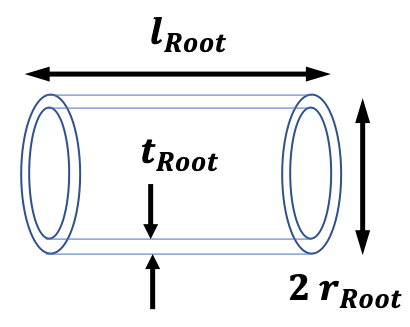
\includegraphics[width=0.4\textwidth]{images/root_fitting.png}
\vspace{-0.1cm}
\caption{Blade root fitting}
\label{fig:root_fitting}
\end{center}
\end{figure}

\subsubsection{Torsion frequency check}
The skin thickness is used to calculate the first elastic torsion frequency for the rotating blade and ensure that it is above 3.3/rev at the hover RPM. If the torsion frequency is too low, then additional skin thickness is added until this requirement is satisfied, preserving the same spar design.

\subsection{Flight controls}
\noindent Two categories of actuators are modeled: fixed-wing, and rotary-wing. 
\subsubsection{Rotor controls}
Unlike large rotorcraft, some eVTOLs feature low-bandwidth collective actuators and no cyclic or swashplate. In such designs, the collective pitch (e.g., for prop-rotors) is usually scheduled with airspeed, and RPM is used for feedback control. Sizing laws for these collective actuators are therefore markedly different from those used for full-scale helicopter controls. The rotor hub mass and collective pitch actuator masses scale with tip speed $V_{\rm TIP}$ (and blade chord $c$ for the actuator) as 
\begin{align}
M_{\rm hub} \spc ({\rm kg})\quad &= \quad 4.84 \left(\frac{V_{\rm TIP}}{171}\right)^2 \left(\frac{c}{0.082}\right) \\
M_{\rm act} \spc ({\rm kg})\quad &= \quad 1.47 \left(\frac{V_{\rm TIP}}{171}\right)^2 \left(\frac{c}{0.082}\right)
\end{align}
The tip speed $V_{\rm TIP}$ is in m/s and mean blade chord $c$ is in meters. 
\subsubsection{Fixed wing controls}
Fixed wing flap and actuator weights are obtained from the AFDD model as 
\begin{equation}
W_{\rm flaps} \spc (lb) \quad = \quad 0.01735 W^{0.644} S_{\rm wing}^{0.41}
\end{equation}
For this model, the weights are in lbs, including the take-off weight $W$. The term $S_{\rm wing}$ is the total plan-form area of all fixed wings, and the actuator weights $W_{\rm flaps}$ includes all actuators on all fixed wings.

\subsubsection{Tilt actuators}
For tilt-rotors and tilt-wing configurations, the masses of tilt actuators are estimated as the larger of 15.5\% of wing mass, and 3.61\% of the total mass being tilted by that actuator. For tilt-wings, both metrics are applicable; for tilt-rotors, the tilt actuator weight is set to 10\% of the masses being tilted.
\begin{align}
M_{\rm tilt-wing} \quad &= \quad \max(0.155 M_{\rm wing}, 0.0361 M_{\rm tilt}) \\
M_{\rm tilt-rotor} \quad &= \quad 0.10 (M_{\rm hub} + M_{\rm act} + M_{\rm blades} + M_{\rm motor}) 
\end{align}

\subsection{Motor mount mass}
\begin{figure} 
\begin{center}
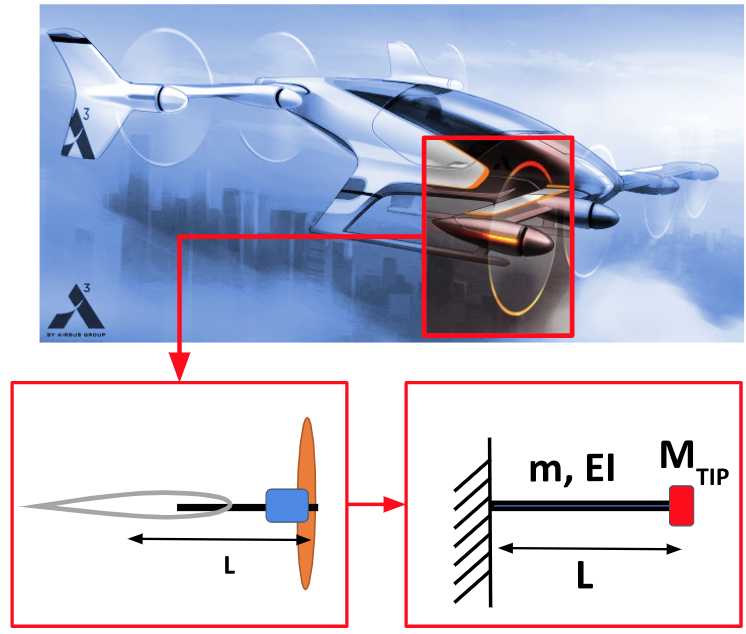
\includegraphics[width=0.6\textwidth]{images/motor_mount.png}
\caption{Motor mount model}
\label{fig:motor_mount}
\end{center}
\end{figure}

The motor mount structure refers to the overhang beam connecting the motor and rotor hub, to a wing (or fuselage). For the Vahana tilt-wing configuration, the motor mount structure is the overhang beam used to offset the rotor hub ahead of the wing leading edge, as shown in Fig.~\ref{fig:motor_mount}. The motor mount is modeled as a cantilever beam of length \textbf{L} with a tip mass equal to the mass of the rotor hub, blades and motor. This structure is sized by a natural frequency requirement, i.e., \textbf{the first cantilever bending mode for this beam with a tip mass} must be sufficiently large so that the structural dynamics do not interact with flight dynamics (0 - 4 Hz). For eVTOLs, a target first bending frequency of 8.5 -- 10 Hz is used to size the motor mount beam. The overhang length is set to the sum of wing three-quarter chord and one rotor radius.

For configurations such as CityAirbus (quad-ducted-coaxial rotors) with no fixed wings, the rotors are mounted directly on the fuselage using support arms. The support arms are treated as ``motor mounts'', and the beam length is set to 120\% rotor radius. Appendix A provides an analytical solution for sizing a cantilever beam with several lumped non-structural masses, distributed structural and non-structural masses based on a target frequency. 

\subsection{Wing weight model}
Three models are available to estimate the weight of a fixed wing:

\subsubsection{AFDD wing weight model}
The weight of a fixed wing is estimated as 
\begin{equation*}
W_{\rm wing} \quad = \quad 5.6641 \frac{\left(\frac{L_w}{1000}\right)^{0.847} n_z^{0.4} S_{\rm wing}^{0.21} AR^{0.5}}{\left(\frac{t}{c}\right)^{0.0936}}
\end{equation*}
The wing weight is in lbs, $L_w$ is the wing design lift in lbs, $n_z$ is the design ultimate load factor, $S_{\rm wing}$ is the wing plan-form area in sq. ft, $AR$ is the wing aspect ratio and $\left(\frac{t}{c}\right)$ is the wing thickness to chord ratio. 

\subsubsection{Frequency tuning: bending loads}
The wing spar is idealized as a cantilever beam with lumped non-structural masses (rotor blades, hub and collective actuator assembly and motor), distributed non-structural masses (skin, ribs) and a hollow circular spar. A schematic of one half-wing is shown in Fig.~\ref{fig:wing_layout}. 

\begin{figure} 
\begin{center}
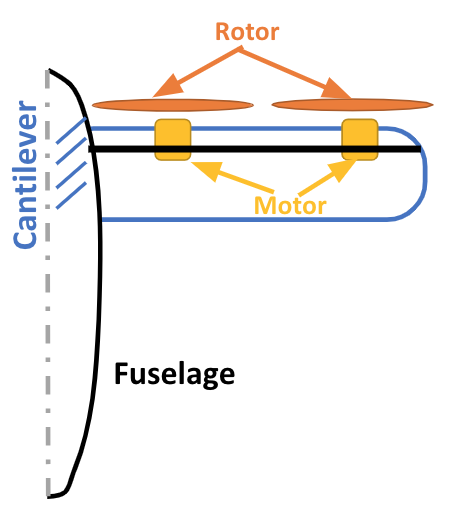
\includegraphics[width=0.35\textwidth]{images/wing_layout.png}
\caption{Wing structure: layout}
\label{fig:wing_layout}
\end{center}
\end{figure}

The wing taper ratio $\lambda$ = $\frac{c_{\rm TIP}}{c_{\rm ROOT}}$ is a design parameter with a default value of 0.75. A tapered wing shifts the non-structural skin mass inboard while strengthening the root, resulting in increased first bending frequency for the same mass. The skin thickness is set to include three layers of carbn fiber (45/0/45), resulting in an areal mass density of $\approx$ 4.9 kg/sq.m. During sizing, the rotor assembly mass and motor mass are used to calculate the wing spar thickness required to achieve a target first bending frequency using the Rayleigh-Ritz approximation detailed in Appendix A. To decouple wing structural dynamics from vehicle flight dynamics, a target first bending frequency of at least 4 Hz is desirable (for a take off mass of 2000 kg). Larger aircraft feature progressively relaxed natural frequency constraints, because the flight dynamic frequencies are lower for larger vehicles with correspondingly larger moments inertia.

\subsubsection{Hover: shear loads}
After determining the spar thickness based on natural frequency requirements, the wing structure is analyzed with static loads in hover with the tapered beam. Rotor thrusts are applied at the motor mount locations and the static bending stresses and shear stresses are calculated at five points between nodes (nodes are located at the root and motor mount locations). A load factor of 3.8 and safety margin of 1.5 are applied to ensure that the spar can support the loads in hover. This hover loading condition is more limiting than cruise flight with the same load factors and safety factors, because the bending moments due to distributed lift are lower than the corresponding bending moments in hover. The shear loading is used to estimate the number of $\pm$ 45 deg layers of carbon fiber, while the bending loads are supported by layers of uniaxial carbon fiber. 

\subsection{Airframe Weight Model}
\subsubsection{Statistical weight model}
The AFDD82 fuselage weight model for helicopter is given by
\begin{equation}
w_{\rm fuselage} = w_{\rm basic} + w_{\rm press} + w_{\rm cw}
\end{equation}
where $w_{basic}$ is the basic weight of the fuselage, $w_{\rm press}$ is the weight from any pressurization constraints (set to none for the sample mission in this work) and $w_{\rm cw}$ is the weight addition for crashworthiness, which is assumed to be 6\% of the basic weight as per AFDD standards. The basic weight is given by
\begin{equation}
\label{eqn:afdd82_fuselage}
w_{\rm basic} = 5.896 f_{\rm ramp} \left(\frac{W_{\rm GTOW}}{1000} \right) ^ {0.4908} n_z ^ {0.1323} S_{\rm body}^{0.2544} l^{0.61}
\end{equation}
where $f_{\rm ramp}$ is the factor for a retractable ramp, $n_z$ is the load factor, $S_{\rm body}$ is the wetted area of the fuselage (sq. ft) and $l$ is the length of the fuselage (feet). While these terms can be defined for full-scale helicopters/tiltrotor, their definitions become increasingly challenging to interpret in the context of unconventional configurations such as an eVTOL, with very different load paths compared to helicopters. %Additionally, even if such a definition can be codified, the error in the model at small take-off weights (less than one ton) is significant (up to 10\% or more). 
\subsubsection{Component build-up model}
Another approach to estimate fuselage mass is to consider the constituent components in the airframe, and estimate the weight of each part based on the design limit loads carried by that part. These parts are 
\begin{enumerate}
\item \textbf{Skin:} using fuselage dimensions and an assumed uniform skin thickness, the skin mass is calculated using the wetted area of the skin. This wetted area is estimated as 
\begin{equation}
S_{\rm wet} \quad = \quad 4\pi \left[\frac{(l_f h_f)^{1.6} \pls (b_f l_f)^{1.6} \pls (b_fh_f)^{1.6}}{3}\right]^{\frac{1}{1.6}}
\end{equation}
The skin consists of paint, core, glue and carbon fiber. The mass of the fuselage skin is therefore
\begin{equation}
M_{\rm skin} \quad = \quad (\rho_{\rm carbon} t_{\rm carbon} \pls \rho_{\rm glue} t_{\rm glue} \pls \rho_{\rm core} t_{\rm core} \pls \rho_{\rm paint} t_{\rm paint})
\end{equation}

\item \textbf{Canopy:} When a canopy is included, the wetted area of the canopy is assumed to be 8\% of the fuselage wetted area, and the canopy mass is calculated as 
\begin{equation}
m_{\rm canopy} \quad = \quad \rho_{\rm canopy} t_{\rm canopy} S_{\rm canopy}
\end{equation}
\item \textbf{Bulkhead:} 4 bulkheads (elliptical cross-sections) are placed along the length of the fuselage. Bulkhead mass is calculated assuming no cut-outs, as 
\begin{equation}
m_{\rm bulkhead} \quad = \quad 4 \left(\frac{\pi bh}{4}\right) t_{\rm bulkhead} \rho_{\rm carbon}
\end{equation}
\item \textbf{Keel beam:} The keel beam mass is estimated based on strength requirements, and sized to carry the following loads: (1) bending moment due to tail lift at a load factor of 3.8 and safety factor of 1.5 (2) torsion moment in the airframe due to differential wing lift of 25\% vehicle weight, and a moment arm of half-span; and finally (3) Combined vertical and lateral shear load during a 3.5 n$_z$ landing.
\end{enumerate}

\subsubsection{Physics-based weight model: load-bearing airframe components}
A physics-based model is used to estimate the weights of load-bearing components that transmit rotor hub forces and wing lift and drag to the vehicle center of mass. The airframe is subdivided into 3-D beam elements, each with bending, axial and torsion degrees of freedom. Rotor hub loads and wing lift/drag are modeled as point loads at the motor points, and distributed uniformly over the wing span, respectively. The external loads corresponding to each mission phase are applied on the structure,  (rotor thrust, torque, wing lift and wing drag) and the resulting stresses and deflections are calculated and stored at all the nodes. Subsequently, the cross-section dimensions of the beams are iteratively resized to ensure; (i) Minimum factor of safety of 1.5 (based on Von-Mises stress) at a load factor of 3.5, (ii) A maximum deflection of 10\% for any node (relative to its distance from the vehicle center). The cross-sections of all beam elements are assumed to be hollow circles with wall thickness equal to 15\% outer radius. The only design parameter for a beam element is the outer radius of the cross-section. Beam cross-section radii for all elements are updated iteratively until the 3 design criteria are satisfied, and the weight of the airframe members is calculated using material density and final dimensions. The finite element analysis iterations are performed within the sizing loop. The parameterization for a quad-rotor layout is shown in Fig.~\ref{fig:airframe}.

\begin{figure}
\begin{center}
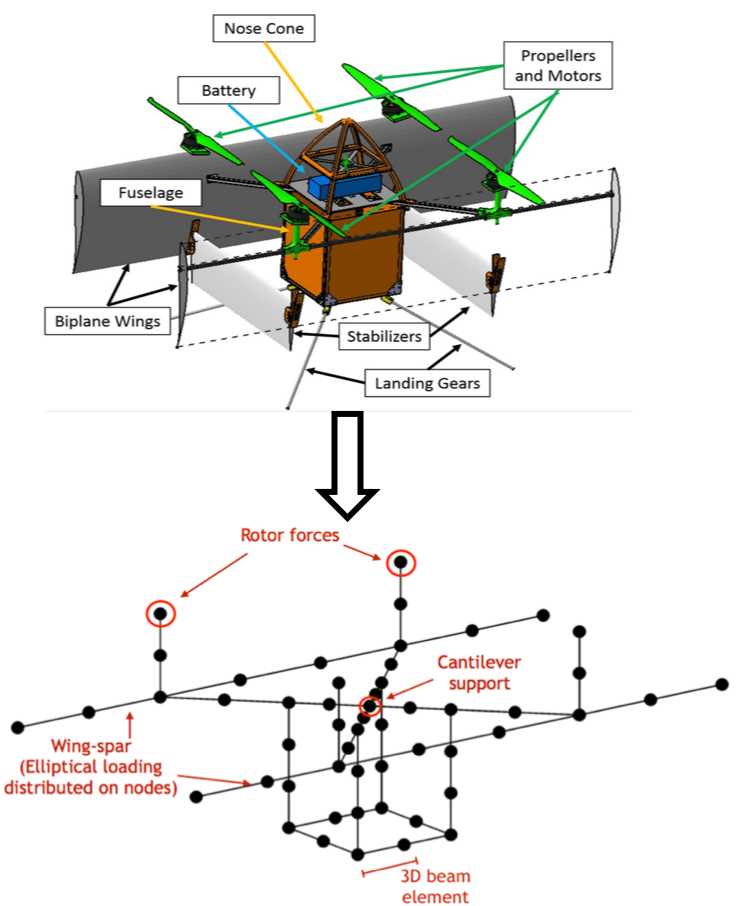
\includegraphics[width=0.65\textwidth]{images/airframe.png}
\vspace{-0.1cm}
\caption{Quad-rotor biplane tail-sitter: layout to finite element representation}
\label{fig:airframe}
\end{center}
\end{figure}

\begin{figure}
\begin{center}
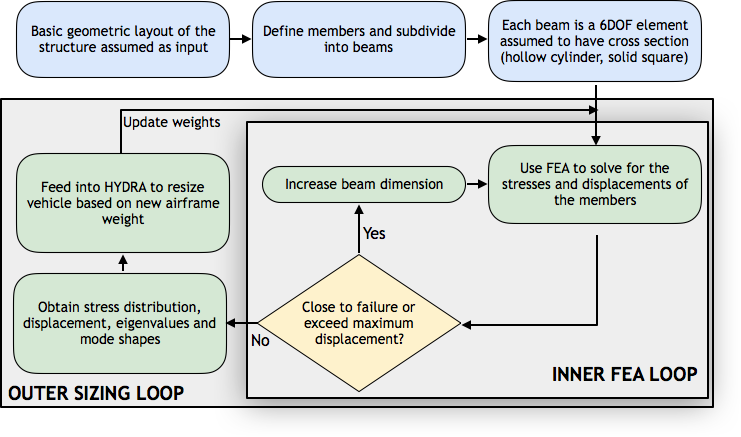
\includegraphics[width=0.75\textwidth]{images/fea_flowchart.png}
\vspace{-0.1cm}
\caption{Workflow for including physics-based airframe weight model in sizing}
\label{fig:fea_flowchart}
\end{center}
\end{figure}

\noindent \textbf{Integration of FEA into sizing: workflow} \\
%In the present work, the airframe is defined as a beam lattice framework and the loads on the structure are computed using a finite element analysis (FEA). The external loads on the structure arise from the weight of different components and the dominant aerodynamics loads (rotor thrust and wing lift). A set of three-dimensional Euler-Bernoulli beam elements with six degrees of freedom at each node (three translations and three rotations) was assembled in a finite element framework. After discretization of the distributed loads into equivalent concentrated forces and moments at wing nodes, the static deflection is obtained and used to compute bending stresses. By requiring each element in the structure to operate within a band of a target safety factor, and not exceed a maximum absolute limit for bending deflection, beam cross-section dimensions are iteratively adjusted in an inner loop within the sizing framework. 
\noindent The overall process is depicted in a flowchart shown in Fig.~\ref{fig:fea_flowchart} and proceeds as follows
\begin{enumerate}
\item {\bf Initialize: } A geometric layout of the airframe is chosen, and beam elements are defined. The present work assumes the beam cross section to be simple shapes such as a hollow cylinder or a solid square.

\item {\bf Inner FEA loop: } Point forces and moments are applied to the structure based on rotor and wing loads, such as rotor thrust, rotor torque and wing lift. The von-Mises stress ($\sigma_{\rm VM}$), the corresponding factor of safety and deflection of the various nodes are computed as
\begin{eqnarray}
\sigma_{\rm VM} &=& [ (\sigma_{xx}-\sigma_{yy})^2 + (\sigma_{yy}-\sigma_{zz})^2   \\ \nonumber
&+& (\sigma_{zz}-\sigma_{xx})^2 + 6(\sigma_{yz}^2+\sigma_{xy}^2+\sigma_{xz}^2) ]^{1/2}
\end{eqnarray}
where $\sigma_{\rm ij}$ are components of the stress tensor and the factor-of-safety (FOS) is
\begin{equation}
{\rm FOS} = {\rm min}(\sigma_{VM})_i / \sigma_{\rm yield} \qquad  \ \forall\ \ i\ \in N
\end{equation}
where $N$ is the total number of beam elements.

\item {\bf Update cross-section dimensions: } The mathematical constraints imposed for convergence are
\begin{equation}
|{\rm FOS}_{\rm tar} - \Delta {\rm FOS}| \leq {\rm min}({\rm FOS})
\end{equation}
% \leq {\rm FOS}_{\rm tar} + \Delta {\rm FOS}
where ${\rm FOS}_{\rm tar}$ is the target FOS, set to 1.5 and $\Delta {\rm FOS}$ is the allowable band, set to 0.1. The axial and bending deflections of each node are normalized by the distance of the node from the vehicle center of gravity. These normalized deflections must not exceed a pre-determined fraction (0.08) to ensure structural rigidity. Depending on the type of condition encountered, two types of cross-section updates are calculated:
\begin{enumerate}
\item The beam cross-section is scaled up by the term (FOS/FOS$_{\rm tar}$)$^{1/3}$) if the factor of safety is not sufficiently large. The cube root in the expression stems from the fact that stress is inversely proportional to cross-section dimension under static load.
\item If the deflection of any one node is too large, the dimensions of all cross-sections are increased by 10\%. Increasing the sizes of all the member cross-sections is required because adding stiffness to the root end of a longer beam may be more effective than stiffening an outboard member (in the present workflow, no apriori assumptions are made about the load path, and so to guarantee deflections are restricted, all members are stiffened).
\end{enumerate}
The larger of the two calculated dimensions for each structural member is provided to the FEA for the next iteration. The stresses and deflections are recalculated, and members resized until the structure achieves the required factor of safety and deflection limits.

The airframe weight is computed by multiplying the total volume of all the beam elements with the material density (Aluminum, 2,700 kg/m$^3$ or carbon, 1650 kg/m$^3$). This converged airframe weight from static finite element analysis replaces the fuselage weight from the AFDD empty weight formulae in the iterative sizing process.

\end{enumerate}
The structural analysis used in in sizing the airframe structure also provides estimates of the natural frequencies and the mode-shapes. This information can be used in advanced stages of design to ensure sufficient separation between the airframe, blade natural frequencies and operating RPM range of the rotor(s). 

\subsection{Weight margin}
A weight margin is included in the analysis to admit additional expansion of component performance (and therefore weight) at later stages of design. Therefore, \textbf{10\% of the vehicle empty weight} is allocated for a weight margin. 

\subsection{Fixed weight groups}
Fixed empty weight groups consist of mission-specific components and do not scale with vehicle dimensions or system performance during sizing. These fixed weight groups are 
\begin{enumerate}
\item Carpets, cabin trim and noise insulation
\item Avionics, sensors and flight computers
\item Airconditioning and heaters
\item Seats
\item Low voltage battery, anti-collision lights, air data systems 
\item High voltage bus and power distributors
\end{enumerate}

\subsection{Comparison of weights vs. NDARC}
To validate the convergence technique, individual weight models and performance models in \hydra, the vehicle weight breakdown was obtained for a single main rotor helicopter with gas turbine engines and a mechanical transmission, and compared to values obtained from NDARC (a NASA sizing code). Table~\ref{tbl:vsNDARC} shows that less than 1\% error is obtained for most groups, while fuel is slight over-predicted by 2.8\%. 

\begin{center}
  \begin{table}[H]
	\caption{Helicopter weight breakdown: \hydra \spc vs. NDARC}
	\label{tbl:vsNDARC}
	\vspace{0.5cm}
    \begin{tabular}{ l | c | c | c }
    \hline
    Group weight (lb) & \hydra \spc prediction & NDARC prediction & \% difference \\ 
    \hline
 Gross weight & 14230 & 14243 & \textbf{0.1\%} \\
Payload & 2500 & 2500 & -- \\
Fuel & 1702 & 1752 & \textbf{2.9\%}  \\
Empty weight & 9252 & 9267 & \textbf{0.16\%} \\
Engine + accessories & 1038 & 1024 & \textbf{1.3\% }\\
Transmission & 1316 & 1292 & \textbf{-1.82\%} \\
Fuel system (pump, tank) & 508 & 505 & \textbf{-0.6\%} \\
Airframe & 1304 & 1301 & \textbf{-0.2\%} \\
Alighting gear & 461 & 463 & \textbf{0.4\%} \\
Rotor system & 1098 & 1100 & \textbf{0.2\%} \\
Empennage & 184 & 179 & \textbf{2.7\%} \\
Flt. control, deicing + hydraulics & 1013 & 1013 & -- \\
    \hline
  \end{tabular}
\end{table}
\end{center}